%\documentclass[12pt,twoside]{report}
\documentclass[12pt]{report}

\usepackage{epsfig}
\usepackage{graphicx}
\usepackage{amsmath}
\usepackage{amssymb}
\usepackage{url}

%% last modification is May 26, 2014, Emma Pease

% note that the document can be single or double sided.  

\usepackage[online]{suthesis-2e}
%\usepackage{suthesis-2e}

    \title{Actionable Information From Electronic Health Records}
    \author{Kenneth Jung}
    \dept{Biomedical Informatics}
    \principaladviser{Nigam H. Shah}
    \firstreader{Mark Musen}
    \secondreader{Lester Mackey \\(Statistics)}
%% one can also have a \thirdreader and \fourthreader

%% note that certain departments and types of theses have other requirements
%% For instance theses in the departments of 
%% Asian Languages
%% French and Italian
%% Spanish and Portuguese
%% need to define the \dept, \dualthesis, and the actual language
%\dualthesis
%\languagemajor{Chinese}
%% 
%% Those for Graduate Program in Humanities need to define 
%\humanitiesthesis
%\jointprogram{Arts and Crafts}
%% 
%% For submission to a committee or program (no department)
% \committeethesis
% \programthesis
%%
%% For School of Education or Business or Law
% \educationthesis
% \businessthesis
% \lawthesis  (law actually isn't listed in the official documents, 2013/1014)

\begin{document}

% for a variety of reasons this is an all in one document; however,
% when actually doing the thesis it is strongly recommended that each
% chapter be in a separate file and use \include to include in the
% main file.

%% the \beforepreface command produces the title/Users/kjung/Dropbox/Nigam/NLP_Compare/Submit/JUNG_JAMIA_MANUSCRIPT_revised_clean.docx page
%% in the online version it skips the copyright (page 2) and signature (page 3) pages 
%% in the non-online version these would be included
    \beforepreface

%% Abstract can be any number of pages
    \prefacesection{Abstract}
Abstract abstract abstract

%% one can also have a prefacesection that is a Preface instead of 
%% Acknowledgements.   The thematic purpose is the same (thanks).  
    \prefacesection{Acknowledgements} 
Ack ack ack

%% afterpreface produces a table of contents and any other tables
%% wanted. At the end pagenumbering changes from roman to arabic and  
%% is restarted 
    \afterpreface 

%% Normally the \chapter and any text would be in a separate file and included.
%    \chapter{Introduction} 
\chapter{Introduction}

\section{Motivation}
Clinicians are often faced with situations in which they must make
decisions with little guidance from medical science.  This situation
has been referred to as the \emph{inferential gap}
\cite{InferentialGap}, and it may arise in many ways.  For instance,
clinicians may be unaware of existing guidelines - it has been
estimated that it takes 17 years on average for findings in clinical
studies to make their way into widespread use \cite{Balas2000}.  It
may also be that the relevant information simply does not exist.

Information from randomized controlled trials (RCTs) is the
gold-standard of evidence of safety and efficacy because, when well
designed and executed, RCTs can control for unobserved confounding
factors.  However, even when those conditions are met, the findings of
RCTs are often difficult to generalize to the sorts of patients seen
in every day practice.  This is primarily due to the sparsity of RCTs
- it is extremely expensive and time consuming to run a randomized
controlled trial.  Driven in part by their expense, RCTs
frequently have strict exclusion criteria that eliminate patients from
study due to age, serious disabilities, co-morbidities, pregnancies
and poly-pharmacy.

Unfortunately, such patients are precisely those that are increasingly
common in actual clinical practice, and account for much of Medicare
and Medicaid expenses.  The end result of this narrow evidence base is
that a shockingly small fraction of clinical decisions are made on the
basis of good evidence that their benefit outweighs their harms.  It
has been estimated that only 11\% of 3,000 comomon clinical
interventions meet this standard in at least the studied population
\cite{BMJClinicalEvidence}.  A review of clinical guidelines issued by
the American College of Cardiology and American Heart Association
similarly found that only 11\% of recommendations in the guidelines
were well supported by strong evidence \cite{Tricoci2009}.  These
estimates of course ignore the issue of whether those recommendations
generalize to other populations.  

Narrowing the inferential gap by broadening the evidence base is one
of the primary goals of the Learning Healthcare System (LHS), defined
in a 2007 Institute of Medicine report \cite{IOM2007LHC,Etheredge2014}
as follows (emphasis added):

\begin{quote}
A learning healthcare system is [one that] is designed to generate and
apply the best evidence for the collaborative healthcare choicees of
each patient and provider; to \emph{drive the process of discovery as a
natural outgrowth of patient care}; and to ensure innovation, quality,
safety, and value in healthcare
\end{quote}

\noindent A cornerstone of the LHS as envisioned by the IOM is the
widespread adoption and interoperability of Electronic Health Record
(EHR) systems \cite{IOMClinicalData}.  The reason for this is simple:
EHRs generate and capture data from routine clinical care rather than
focussing on narrow populations and disorders, as is the case in most
clinical trials.  Thus, widespread use of EHRs has the potential to
provide a more comprehensive picture of the diagnosis, treatment, and
outcomes of the entire population, and to do so in a timely manner,
than other data sources such as administrative (e.g., insurance
claims) data.  The discovery of knowledge derived from this such data
sources has been called \emph{Practice Based Medicine} and it turns
the paradigm of Evidence Based Medicine (EBM), in which data is
generated through a top down process, on its head by embedding the
first stage of knowledge discovery in routine care
\cite{Embi2013,Weng2012,Shah2012}.

The Health Information Technology for Economic and Clinical Health
(HITECH) Act, part of the 2009 American Recovery and Reinvestment
Act (ARRA), authorized \$20 billion in spending over five years to
incentivize the adoption and \emph{meaningful use} of EHRs.  It is
hoped that the increased scope of data generation and capture will be
transformative for addressing questions of treatment efficacy, safety,
quality of care, and comparative effectiveness.  Although it remains
challenging for many health care institutions to meet the criteria
laid out by the HITECH Act for meaningful use, 59\% of US hospitals
had at least a basic EHR that implemented 10 basic functions defined
by the Office of the National Coordinator for Health Information
Technology \cite{AdlerMillstein2014}, compared with 11\% in 2009.  

However, there are many obstacles on the path from the use of EHRs to
achieving the ``best care, at lower cost'' that is the aim of the
IOM's vision.  In this work, we focus on the thorny issue of how
exactly to take advantage of the data in EHRs, most of which resides
in the unstructured text of clinical notes (\textbf{best ref?}), to
generate actionable information that is of use to clinicians and other
agents of the health care system.  Specifically, we pose several
questions that are of immediate clinical interest and demonstrate how
data from EHRs collected during routine care can be used to address
them.

\section{Outline}
We present work that demonstrates that it is possible to extract
actionable information from data in EHRs collected during routine
patient care.  One set of studies focuses on the free text of clinical
notes, and use 9 million notes from the Stanford Translational
Research Itegrated Database Environment (STRIDE) \cite{Lowe2009} as
their primary data source.  These studies show that it is possible to
address a variety of questions in the domain of drug safety with
simple, highly scalable methods.  The key to this scalability is
performing learning at the level of abstract concepts of interest -
i.e., drugs and indications, rather than individual notes.  This
allows use to eschew computationally expensive detailed linguistic
analysis of the text.  The first study addresses how to use the
unstructured free text from EHRs to discover off-label drug use.  A
closely related study turns to how to use free text to discover
drug-adverse events.  The next set of experiments evaluates the
trade-off between simple, highly scalable text mining methods and more
complex methods.  Specifically, for the types of drug safety questions
we study, is there a benefit to using the more complex systems?
Finally, we study the use of EHR data from a different setting -
outpatient wound care centers operated by Healogics Inc - to build
accurate, well calibrated predictive models of delayed wound healing.
We also explore the consequences of non-stationarity on these
models. Below we briefly describe each study and their key findings.

\subsection{Discovery of Off-label Drug Use from Clinical Text}
Off-label drug use, defined as use of a drug in a manner that deviates
from its approved use as defined by the drug's FDA label, is
problematic because such uses have not been evaluated for safety and
efficacy.  Studies estimate that 21\% of prescriptions are off-label,
and only 27\% of those have evidence of safety and efficacy.  We took
a data-mining approach to systematically identify off-label usages
using free text notes from STRIDE, along with domain knowledge
extracted from two databases of known usages (Medi-Span and DrugBank).
We validated 403 putative novel off-label usages across independent
datasources and prioritized well-supported novel usages for further
investigation on the basis of drug safety and cost.  This study
demonstrates the feasibility data mining approaches to using free text
from EHRs to address a question of significant clinical interest.

\subsection{Discovery of Adverse Drug Events from
  Clinical Text}
Adverse drug events (ADEs) are undesired harmful effects resulting
from use of a medication,and occur in 30\% of hospitalized patients.
We used a data-mining approach to systematically identify ADEs using
the free text of STRIDE, along with prior knowledge of drug usages and
adverse drug events.  Putative ADEs are further filtered for support
in two independent, complementary data sources.  This method is
evaluated by assessing support for the predictions in other curated
data sources, including a manually curated, time indexed reference
standard of FDA label change events.  We find that 35\% (87 of 240
high-confidence, well-supported ADEs) are supported by at least one of
these resources.  This demonstrates the feasibility of systematic
post-marketing surveillance for ADEs using free text from EHRs.  

\subsection{Functional Evaluation of text-mining tools for clinical
  data mining tasks}
The above studies beg the question of whether or not it would be
advantageous to use a more sophisticated text processing system.  
The trade-off between the speed and simplicity of dictionary-based
term recognition and the richer linguistic information provided by
more advanced Natural Language Processing (NLP) is an area of active
discussion in clinical informatics.  In this study, we systematically
evaluate this trade-off using the NCBO Annotator and REVEAL, a
commercial system based on MedLEE.  We first benchmarked these systems
on a manually annotated, publically available dataset from the 2008
i2b2 Obesity Challenge.  We then performed a functional evaluation of
the systems in three clinical research tasks: phase IV safety
profiling of a drug, learning adverse drug-drug interactions, and
learning used-to-treat relationships between drugs and indications.
We show that there is no significant difference in between the NCBO
Annnotator and REVEAL with respect to these tasks.  This shows that
there is a large class of problems of direct clinical relevance which
are addressable by current, highly scalable text mining methods.

\subsection{Predictive models of delayed wound healing}
Finally, we explore the use of EHR data for fitting predictive models
in the context of wound healing in outpatient wound care centers.  The
outcome of interest in this study is whether or not a given wound will
take an unusually long time to heal, using information available in
the EHR during the first week of care.  Our goal in these experiments
is two-fold.  First, we want to fit accurate, well-calibrated models
for delayed wound healing.  We find that it is indeed possible to fit
such models.  Second, we note that the dataset we use in this study
shows a significant degree of non-stationarity arising from a variety
of sources.  We believe that this situation is likely to be mirrored
on many other datasets derived from EHRs during this period of
remarkable changes in the health care system.  Thus, we also explore
the impact of non-stationarity on model development and evaluation.
We simulate varying degrees of non-stationarity by using different
procedures to split the dataset into training and test sets.  We are
able to fit accurate, well calibrated models but also find that specific
conclusions about model selection and generalization error are
complicated by non-stationarity in the dataset.  





\chapter{Learning Off-label Drug Usages}

\section{Introduction}
Off-label drug use occurs when a drug is used in a manner that differs
from its approved use as described by its FDA label.  This practice is
common and provides a pathway for clinical innovation.  However, such
uses escape the scientific scrutiny that goes into the labeling and
marketing of new medicines \cite{Stafford2012,Pan2012}.  Estimates
from office-based practices found that 21\% of prescriptions are
off-label .  Of these, 73\% had little or no scientific support
\cite{Radley2006,Chen2009}, raising concerns about patient safety and
costs to the healthcare system.  For instance, tiagabine was approved
for use as an adjunctive therapy for partial epilepsies.  However,
when used as the sole or primary treatment, it was found to cause
seizures.  In 1998, 20\% of uses of tiagabine were off-label, but by
2004 this fraction had increased to 94\% \cite{Flowers2006}.

Off-label use is to some extent inevitable because not every condition
can be tested during pre-approval \cite{Kimland2012,Epstein2012}.
Nevertheless, all stakeholders in the health care system have an
interest in the timely, systematic detection of off-label use.  Drug
manufacturers are required to report on off-label use observed in
post-marketing surveillance in the European Union \cite{Morris2012}.
Regulatory agencies and clinical researchers can use knowledge of
emerging off-label uses to identify potential benefits or risks that
require further investigation.  Furthermore, patients and their health
care providers should minimize exposure to risks without clinical
benefit.  Unfortunately, current pharmacovigilance and post-market
surveillance efforts in the United States do not monitor off-label
use.  Standard surveillance approaches using the FDA's Adverse Event
Reporting System (FAERS) do not specifically account for use in
off-label indications; efforts such as the Observational Medical
Outcomes Partnership (OMOP) and the Mini-Sentinel projects do not
specifically look at off-label use \cite{Platt2012}; and physician
surveys, such as the NDTI, are limited by coverage, timeliness and
cost.

In this work, we focus on the problem of automatically discovering
off-label uses of drugs—defined as the use of drugs for unapproved
indications—from electronic health records and rank the newly
discovered uses for follow up based on risk and cost metrics.  At its
core, we need to match drugs to the diseases they are being used to
treat.  We refer to such matches as drug-indication usage pairs, and
say that a used-to-treat relationship exists between the drug and
disease (the indication).

Previous work by Wei et al \cite{WeiQi2013} used structured and
semi-structured data from RxNorm, MedlinePlus, SIDER 2, and Wikipedia
to compile a comprehensive list of drug-indication usage pairs.
Similarly, Xu et al \cite{Xu2013} used data from ClinicalTrials.gov
and Medline to compile such a list.  However, both these efforts rely
on curated data sources that may not reflect current clinical
practice.  In contrast, the data in electronic health records
represents current clinical practice and can discover such usages
before they are incorporated into curated data sources.

Thus, widespread adoption of electronic medical records (EMR) provides
an opportunity to detect off-label use in an automated, scalable and
timely manner \cite{Morris2012}.  However, structured data in EMRs
usually do not explicitly link diseases to the drugs being used to
treat them \cite{Pan2012} and is not as comprehensive as the free text
of clinical notes \cite{Poissant2010}.  Therefore, Natural Language
Processing (NLP) is often used to extract used-to-treat relationships
between drugs and indications from clinical text.  Previous efforts
use one of two approaches: the first approach identifies used-to-treat
relationships at the level of specific occurrences of drugs and
indications in text.  For example, from the phrase, “on Plavix for
PAD”, a used-to-treat relationship between clopidogrel and peripheral
artery disease is detected.  Submissions to the 2010 i2b2 NLP
Challenge \cite{Uzuner2011} represent the state of the art of this
approach.  The best performing methods require examples of text in
which occurrences of drugs, indications and the relationships between
them are explicitly labeled \cite{Chapman2011}. Such labeled training
data is difficult to obtain (the i2b2 Challenge included 871 labeled
notes) and collections of labeled text covering all drugs and
indications are not available. To overcome this limitation, an
alternative approach is to infer used-to-treat relationships at the
population level—rather than asking whether a sentence or note implies
an instance of a used-to-treat relationship, we ask whether the data
as a whole suggests that a used-to-treat relationship holds in general
\cite{Chen2008,Rindflesch2005,Lependu2012}.  The basic idea is to
count the number of times a drug and indication are mentioned in the
same clinical record, and compare that count to the expected
co-mentions by chance.  We have previously used such an approach for
detecting drug-related adverse events \cite{Lependu2013}, identifying
drug-drug interactions \cite{Iyer2013}, and profiling drug usages
\cite{Lependu2012}.  Such approaches can use relatively simple,
methods for detecting drug and indication mentions in free text that
do not require labeled text corpora for training.  As a result, such
approaches scale to very large collections of clinical text and the
entire range of drugs and indications encountered in the data.  In
Jung et al \cite{Jung2013}, we demonstrated that it is possible to
detect off-label usage using inputs derived from clinical text,
combined with prior knowledge of drugs and indications from Medi-Span
and DrugBank.  Other researchers \cite{Li2011} have also used prior
knowledge of known usages to match drugs and known indication mentions
in clinical notes demonstrating that use of prior knowledge does
improve the accuracy of detecting used-to-treat relationships.

In this paper, we build on our previous work. First, we have improved
the accuracy of the classifier by taking known usage into account when
counting co-mentions of drugs and indications in the clinical notes in
order to reduce spurious associations arising from co-morbidities.
Second, we have filtered the set of predicted novel off-label usages
for support in independent, complementary data sources.  We also
filtered out spurious associations due to causal relationships using
the SIDER 2 database \cite{Kuhn2010}.  Finally, in order to triage the
off-label uses for follow-up, we developed indices of drug cost and
risk associated with a drug’s usage based on the unit price and known
adverse events of drugs.  These indices were used to rank off-label
usages by the risk that they present to patients, along with their
monetary cost.  High cost and high risk usages are natural candidates
for further investigation as they represent expensive and potentially
dangerous cases.  Whereas, low cost and low risk usages could be
potential expanded indications.  Our methods do not require labeled
training text, and thus combine the scalability of association-based
approaches with the discriminative power of machine learning
techniques.  The overall approach and results are summarized in Figure
2.1.

\begin{figure}
  \begin{center}
    \includegraphics[width=0.9\linewidth]{ch2-figures/Figure1.pdf}
  \end{center}
  \caption[Overview of learning off-label usages]{Overview of methods
    and results.  For each of the 2,362,950 possible drug-indication
    pairs, we calculated 9 empirical features (e.g., co-mention count)
    from the free text of clinical notes in STRIDE and 16 domain
    knowledge features (e.g., similarity in known usage to other drugs
    used to treat the indication) from Medi-Span and Drugbank.  These
    features were used by an SVM classifier trained on a gold standard
    dataset to recognize the used-to-treat relationship, yielding a
    set of predictions that were filtered for known usages, near
    misses in the indications, and support in two independent and
    complementary datasets (FAERS and MEDLINE).  Predicted usages that
    appeared to be drug adverse events listed in SIDER 2 were removed.
    The resulting set of 403 well-supported novel off-label usages
    were binned using indices of risk and cost.  }
  \label{fig:short}
\end{figure}


\section{Materials and Methods}
\subsection{Constructing a gold standard}
We constructed a gold standard of positive and negative examples of
drug usage using known usages from Medi-Span. Medi-Span contains
13,453 drug-indication pairs comprising 1,642 unique drugs and 2,313
unique indications.  Of these, 1,602 of the drugs and 1,475 of the
indications occur in STRIDE at least once, yielding a set of 8,861
testable drug-indication pairs.  To construct negative examples, we
sampled known usages from Medi-Span with replacement and then sampled
new drugs and indications that occur in the data with approximately
the same frequency.  For instance, given the known usage
“dexamethasone for systemic lupus erythematosus”, we sample a new drug
from the set of drugs that occur within ten items of dexamethasone in
a list of drugs sorted by overall frequency in the data.  A new
indication is similarly generated from systemic lupus erythematosus.
Frequency matching was done because previous work suggested that
frequencies can help distinguish between drug associated adverse
events and treatment relationships \cite{Liu2012}.  The "negative"
pairs were filtered to remove inadvertent known usages.  The final
gold standard consisted of 34,974 negative and 8,861 positive
examples.

\subsection{Annotation of clinical text from STRIDE}
We used the NCBO Annotator on free text of 9.5 million clinical notes
from STRIDE to annotate the each note with mentions of drugs and
indications in terms of UMLS \cite{Bodenreider2004} unique concept
identifiers (CUI's).  Negated mentions (e.g., “MI was ruled out”) or
those referring to other people (e.g., “father had a stroke”) were
removed using NegEx \cite{Chapman2001} and ConText \cite{Chapman2007},
respectively.  Drugs were normalized to 1,602 unique active
ingredients (e.g., Excedrin was rewritten into acetaminophen, aspirin
and caffeine) using RxNorm \cite{Nelson2011}.  Indications were
normalized to the set of 1,475 indications used in Medi-Span by
recursively rewriting the indication as its parents in the SNOMED CT
hierarchy until we reached an indication used by Medi-Span.  For
instance, ‘amok’ is not in the Medi-Span target vocabulary so it is
rewritten as its parent term, ‘mania.’ We note that if the mentioned
indication is an ancestor of the known indication, it may be counted
as a novel off-label usage later on.  We consider this to be
reasonable because if the detected usage is broader than the known,
approved usage, it is indeed off-label provided the terms are used
precisely as intended.  In reality, terms are not used so precisely,
so we allow for some imprecision in the usage of terms when filtering
out known usages from predicted usages as described below.  The
clinical notes covered 1.6 million patients and spanned 18 years of
data, and included all clinical notes generated for these patients at
Stanford Hospital during that time.

\subsection{Feature Construction}
For each patient, a drug or indication is counted as present if they
appear in any of the patient’s notes.  They count as co-occurring if
they are both mentioned in the patient’s notes and there is no other
indication mentioned in the record that is a known usage for the drug;
all co-occurrences of known indications are also counted.  Doing so
ensures that a drug (e.g. Lisinopril) does not get associated with a
disease (e.g. Diabetes) just because the disease is a common
co-morbidity of the drug’s actual indication (e.g. Hypertension).  In
this process, known usage is defined as appearing in either Medi-Span
or NDF-RT. These counts, along with derived association measures (chi
squared statistic, odds ratio and conditional probability of drug
mention given indication mention), were used as features. The fraction
of patients in which the drug occurs before the indication (drug first
fraction) was also included, along with drug first fractions adjusted
for frequency of the drugs and indications \cite{Liu2012}. Overall, we
used nine features encoding the pattern of mentions of the drugs and
indications in clinical text.

We also used features that encode prior knowledge of the drugs,
indications and known usage.  These features were motivated by the
intuition that drugs are typically used off-label because of some
similarity with an approved drug, such as a shared molecular target,
pathway or drug class \cite{Epstein2012}.  We used the Medi-Span and
DrugBank databases to construct features for each drug-indication
pair.  For Medi-Span, these included the number of drugs approved or
known to be used for the indication, the fraction of known treatments
for the indication that are approved, the similarity of the drug to
drugs known to be used for the indication, and the similarity of the
indication to other indications treated by the drug. Drug-drug
similarity features were calculated as described in Figure 2.2.
Indication-indication similarities were calculated similarly, with the
role of the drugs and indications reversed.  When calculating these
features, we ignored known usages that were in the test set to avoid
contaminating the training data with knowledge of test usages.

\begin{figure}
  \begin{center}
    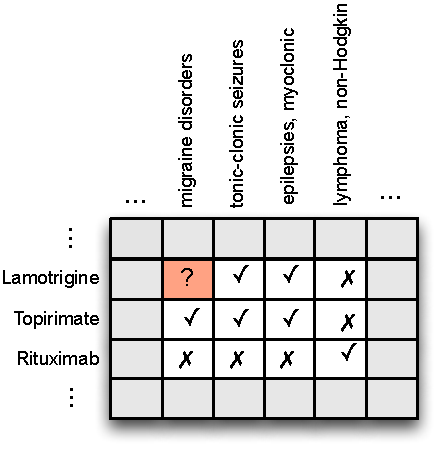
\includegraphics[width=0.6\linewidth]{ch2-figures/Figure4.pdf}
  \end{center}
  \caption[Using prior knowledge to calculate drug-drug and
    indication-indication similarity]{Using prior knowledge to
    calculate drug-drug and indication-indication similarity.  We
    represent known usage as a matrix where row i represents drug i
    and column j represents indication j.  A check in entry (i,j)
    indicates that the drug i is used to treat the indication j, while
    a cross indicates the converse.  We are interested in whether a
    given drug, lamotrigine, is used to treat migraine disorders.  We
    thus ask — how similar is the known usage of lamotrigine to other
    drugs we know are used to treat migraine disorders?  Topirimate is
    used to treat migraine disorders, and lamotrigine is similar to it
    in that both are used to treat tonic-clonic seizures and myoclonic
    epilepsies, but not non-Hodgkin's lymphoma.  This similarity in
    usage profile suggests that it is more likely to be used to treat
    migraine disorders than, say, Rituximab.  We measured this
    similarity using the maximum cosine and Jaccard similarity of
    lamotrigine versus all drugs known to treat the indication.  We
    calculate the similarity between indications based on known usage
    using the same data, with the roles of drugs and indications
    reversed.}
  \label{fig:short}
\end{figure}

The DrugBank 3.0 \cite{Knox2011} database provides information on
6,711 drugs and their molecular targets, pathways, and indications.
The annotator was used to map DrugBank drug names and indications to
our target sets of drugs and indications. Molecular targets, pathways,
and drug categories were also extracted for each drug.  We calculated
similarity features analogous to the Medi-Span similarity features,
along with other features that capture similarity with respect to
molecular targets, pathways, and drug categories.  As with the
Medi-Span derived features, we removed test usages from DrugBank
before calculating features.  

\subsection{Training a predictive model}
The gold standard dataset was randomly split into 35,050 training and
8,784 test examples.  We trained an SVM classifier using radial basis
function kernels on the training examples using the e1071 library in
R.  The performance of the classifier was tested on the test examples.
We also trained and tested classifiers using subsets of the features
to assess the contribution of different groups of features.  We then
trained a classifier on the entire gold standard and applied it to all
2,362,950 possible drug-indication pairs.  In all cases, we used
ten-fold cross validation on the training data and the “1-se” rule to
select the cost hyperparameter for the SVM models.  Estimates of each
prediction’s class membership probabilities were obtained via logistic
regression \cite{Platt1999}.  We used a probability threshold of 0.99
in order to limit the set of predicted usages to the most confident
predictions.  This hard threshold was not tuned in any way; thus our
final set of predicted novel off-label usages could possibly be
improved by adjusting this threshold.  However, this is a very simple
way to restrict our attention to the most confident predictions.

\subsection{Identifying known usages}
Known usage was determined by presence in Medi-Span or the NDF-RT –
drug-indication pairs absent from both are assumed to be novel usages.
Review of these usages revealed that indications were sometimes
closely related to known usages — e.g., glaucoma and open angle
glaucoma.  We addressed this problem using biomedical ontologies,
which organize biomedical concepts into hierarchies — e.g., amok is a
subtype of the parent concept mania.  Specifically, we removed
predicted usages in which the indication is a subtype of a known usage
indication in SNOMED-CT, or is the direct parent of a known usage
indication in SNOMED-CT.  As a final check against Medi-Span and
NDF-RT, we manually reviewed predicted usages remaining after
validation in FAERS, MEDLINE and SIDER2 (described below), removing 63
usages that were not detected as known usages by the methods described
above.

\subsection{Validation by FAERS, MEDLINE and mechanistic plausibility}
FAERS case reports contain explicit used-to-treat links between drugs
and indications.  We validated predicted usages using these links
using public domain case reports from Q3 2007 through Q2 2012.  FAERS
drugs and indications were mapped to UMLS CUI’s, yielding a set of 3
million drug-indication reports covering 160,989 unique pairs.  Only
3,756 out of 8,861 (43\%) positive examples of drug usages in our gold
standard dataset appear at least once in FAERS.  We required at least
10 such reports because this threshold results in a false positive
rate of less than 0.005 when applied to the gold standard dataset.

MEDLINE entries are manually annotated with MeSH terms, Supplementary
Concepts for drugs, and subheadings that provide further context for
the annotation.  For instance, an article about treatment of wet
macular degeneration by bevacizumab would be annotated with “wet
macular degeneration/drug therapy*” and, separately, “bevacizumab.”
We downloaded the complete set of annotations for MEDLINE entries from
2002-2012.  MeSH annotations were filtered for indications with the
drug therapy sub-heading and mapped to UMLS CUI’s using the NCBO
Annotator.  The Substance annotations were also mapped to UMLS CUI’s
using the Annotator.  If no MeSH term corresponded exactly to the
indication, we expanded the indication to the more general MeSH term,
e.g., ‘malignant neoplasm of the ovary’ was interpreted as ‘ovarian
neoplasm’.  As in Avillach et al \cite{Avillach2013}, we considered
usages with at least three articles annotated with both the indication
and the drug to be well-supported by MEDLINE.

We assessed the mechanistic plausibility of predicted usages by
examining patterns of gene expression induced by the drug and
indication.  Briefly, we performed gene set enrichment analysis on
gene expression data from the NCBI Gene Expression Omnibus (GEO)
\cite{Edgar2002} and the Connectivity Map \cite{Lamb2006} to identify
biological pathways and expression modules that are inversely
regulated between pairs of diseases and drugs, suggesting a possible
basis for a therapeutic association \cite{Sirota2011}.  

\subsection{Removal of drug adverse events}
We used drug adverse events listed in the SIDER 2 resource to minimize
the impact of confounding causal relationships on our results.  67 out
of 406 novel, well-supported off-label usages matched SIDER 2 entries.
However, manual review of these matches revealed that only 28
drug-indication pairs were likely to be bona fide drug related adverse
events.  This is due to the fact that SIDER 2 is not curated and thus
includes many spurious results such as indications being listed as
adverse events.  After removal of the true adverse events, 403
off-label usages remained.  Calculation of risk and cost indices The
cost and risk indices are motivated by the observation that off-label
usages do not all have the same urgency for further investigation.
Decision analysis suggests that we rank usages based on their expected
utility — i.e., the desirability of possible outcomes of the use,
weighted by the probability each outcome \cite{Meltzer2011}.  For
example, the use of a cheap antibiotic with few side effects to treat
a rare condition has a lower urgency for follow-up than the use of an
expensive drug, with severe side effects, to treat a common disorder.
We approximated this approach by developing quantitative indices of
drug cost and risk associated with drug usage based on known adverse
events

The cost index was calculated by ranking drugs by their mean unit cost
in Medi-Span (a drug may have multiple unit costs due to different
formulations, etc.).  The ranks were normalized to lie between 0 and
1, with the most expensive drug having a score of 1.  The risk index
for each drug was based on an estimate of the expected disutility of
adverse events associated with using that drug in Medi-Span. Briefly,
we assigned quantitative disutility values to adverse events
associated with drugs in Medi-Span.  The expected disutility of drug
use due to adverse events was then estimated as the weighted sum of
the disutilities for associated adverse events, with the weights given
by probabilities estimated from Medi-Span’s estimates of the frequency
of the adverse events.  Drugs were ranked by expected disutility and
the ranks normalized to lie between 0 and 1 such that the riskiest
drug had a value of 1. The lower and upper quartiles of the cost and
risk index values observed in the 403 well-supported novel usages were
used as thresholds for defining high and low risk or cost groups.

\section{Results}
We trained an SVM classifier to recognize used-to-treat relationships
between drugs and indications and applied the classifier to all
possible drug-indication pairs.  Filtering for high prediction
confidence yielded 14,174 high confidence used-to-treat
relationships. We then removed known usages listed in two curated
sources of known usage — Medi-Span and the National Drug File –
Reference Terminology (NDF-RT) \cite{Brown2004}, leaving 6,142
predictions that could be novel off-label usages.  We assessed support
for the putative novel off-label uses in independent and complementary
data sources including the FDA’s Adverse Event Reporting System
(FAERS) and MEDLINE.  When possible, we also assessed the biological
plausibility of these usages using publically available gene
expression data \cite{Sirota2011}.  We reduce spurious results arising
from drug adverse events by filtering these usages using SIDER 2,
yielding a final set of 403 well-supported novel off-label
usages. Overall, we tested 1,602 unique drugs and 1,475 unique
indications, resulting in 403 well-supported novel off-label usages
that we prioritized by their potential risks and cost.

\subsection{A classifier for detecting used-to-treat relationships}
Classifiers such as support vector machines map inputs, or features,
to outputs.  In this study, the inputs come from clinical text and
domain knowledge about drugs from Medi-Span and DrugBank.  Medi-Span
encodes information about know usages, while Drugbank encodes
information about drug targets and mechanisms of action.  For each
drug–indication pair, we construct a set of features that the
classifier uses to predict whether a used-to-treat relationship holds
between the drug and indication.  The classifier learns to make
accurate predictions using inputs for which we know the desired
output, i.e., positive or negative examples of known usages
\cite{Hastie2009}.  We constructed such a gold standard dataset of
known usages from the Medi-Span Drug Indications Database (Wolters
Kluwer Health, Indianapolis, IN) as positive examples, along with
negative examples constructed as detailed in Methods.  An SVM
classifier was trained on a random subset (80\%) of the gold standard
and achieved a positive predictive value of 0.963, specificity of
0.991, sensitivity of 0.764 and F1 score of 0.852 on the remaining
20\% of the gold standard (see Figure 2.3).  Feature ablation
experiments showed that each group of features contributed to overall
performance, particularly with respect to sensitivity and positive
predictive value (Table 2.1).  Individually, the features learned from
clinical notes in the Stanford Translational Research Integrated Data
Environment (STRIDE) and Medi-Span yielded sensitivities of 0.681 and
0.662 respectively, while all features together resulted in a
sensitivity of 0.764.  In identifying population level associations,
drugs and diseases may also get associated because of causal
relationships (i.e., the drug is causing the disease, as an adverse
drug event) or indirect relationships (i.e., the disease is a common
co-morbidity of an approved indication) rather than used-to-treat
relationships.  We count co-mentions of drugs and indications taking
known indications into account, and as a result, obtain substantially
better performance than previous methods that ignore known indications
\cite{Jung2013}.  Similarly, the PPV achieved using all features was
0.963, substantially better than the 0.936 achieved using only
features derived from just STRIDE and consistent with the hypothesis
that prior knowledge is able to reduce spurious results arising from
causal and indirect relationships \cite{Li2011}.

\begin{table}
\begin{center}
\begin{tabular}{|c|c|c|c|c||}
  \hline Feature set & PPV & Specificity & Recall & F1 \\ \hline\hline
  Naive STRIDE only & 0.771 & 0.964 & 0.483 & 0.594 \\ STRIDE only &
  0.936 & 0.988 & 0.681 & 0.788 \\ Medi-Span only & 0.945 & 0.990 &
  0.692 & 0.778 \\ Drugbank only & 0.831 & 0.981 & 0.377 & 0.518
  \\ STRIDE + Medi-Span & 0.967 & 0.994 & 0.744 & 0.841 \\ STRIDE +
  Drugbank & 0.936 & 0.988 & 0.697 & 0.799 \\ All & 0.963 & 0.993 &
  0.764 & 0.852 \\ \hline
\end{tabular}
\end{center}
\caption[Performance of used-to-treat classifier]{Performance of
  classifier on hold-out test set using different feature sets.  We
  performed feature ablation experiments to assess the contribution of
  different feature sets to the performance of the classifier for
  detecting used-to-treat relationships.  The first column indicates
  the features used to train and test the classifiers.  Classifier
  performance was evaluated in a hold out test set of 1,749 positive
  and 7,035 negative examples of drug usage after training in a set of
  7,112 positive and 27,938 negative examples.  The first row shows
  performance using STRIDE derived features in which co-mentions are
  counted without regard to present known indications in the clinical
  record.}
\end{table}


\begin{figure}
  \begin{center}
    \includegraphics[width=0.9\linewidth]{ch2-figures/Figure2.pdf}
  \end{center}
  \caption[Training a classifier to recognize used-to-treat
    relationships]{Training and testing a classifier to recognize
    used-to-treat relationships.  We created a gold standard of
    positive and negative examples of known drug usage.  Positive
    examples were taken from Medi-Span.  We created negative examples
    by randomly selecting positive examples and then randomly choosing
    a drug and indication with roughly the same frequency of mentions
    in STRIDE as the real usage.  These were then checked against
    Medi-Span to filter out inadvertently generated known usages.  The
    gold standard dataset contained 4 negative examples for each
    positive case.  For each drug-indication pair in the gold
    standard, we calculated features summarizing the pattern of
    mentions of the drugs and indications in 9.5 million clinical
    notes from STRIDE. We used Medi-Span and Drugbank to calculate
    features summarizing domain knowledge about drugs and their
    usages.  80\% of the gold standard was used to train an SVM
    classifier, and the resulting model was tested on the remaining
    20\%.  }
  \label{fig:short}
\end{figure}


\subsection{Predicting novel off-label usages}
We applied an SVM trained on the entire gold standard dataset to all
2,362,950 possible drug-disease pairs to find used-to-treat
relationships.  SVMs do not output class membership probabilities;
thus we fit a logistic regression model to the output of the SVM to
estimate the probability of the used-to-treat relationship being true
for a given drug-disease pair \cite{Platt1999}.  Applying a cut-off of
0.99 to this estimate yielded 14,174 high confidence used-to-treat
relationships, which we interpret as potential drug-indication usage
pairs.  After filtering out known usages listed in Medi-Span and the
National Drug File – Reference Terminology (NDF-RT) \cite{Brown2004},
we removed usages in which the predicted indication is closely related
to already known indications as described in Methods, resulting in
6,142 high confidence novel usages.  Because approved usages are
presumably known, these are interpreted to be high confidence novel
off-label usages.

\subsection{Support in FAERS, MEDLINE and SIDER 2}
The 6,142 high confidence novel off-label usages were examined for
positive support in two independent and complementary data sources
(FAERS and MEDLINE) and for negative support in SIDER 2 as described
in Methods.  FAERS case reports explicitly link indications and the
drugs used to treat them \cite{WeissSmith2011}.  These reports are
created by patients, health care providers and drug manufacturers, and
directly reflect clinical practice.  In contrast, MEDLINE provides
curated annotations of the biomedical literature with terms from the
National Library of Medicine’s Medical Subject Headings (MeSH)
vocabulary.  We found that 766 novel off-label usages are supported by
at least 10 records in FAERS, and 537 of those are also supported by
at least two articles co-annotated with the drug and indication in
MEDLINE \cite{Avillach2013}.  We then filtered out usages that
appeared to be bona fide drug adverse events listed in SIDER 2 in
order to eliminate drug-disease pairs that are actually drug-adverse
event relationships, leaving us with 466 candidate novel off-label
usages.  We manually examined these to filter out known usages that
were missed in Medi-Span and the NDF-RT, leaving us with 403
well-supported novel off-label usages.

These usages cover 210 drugs and 184 indications, and recapitulate
previously noted patterns of off-label usage (Figure 2.4).  Medical
specialties such as oncology have been noted to have high rates of
off-label usage \cite{Poole2004}. Consistent with this observation,
there are many cancer drugs among our results — e.g., ofatumumab for
non-Hodgkin’s lymphoma \cite{Hagenbeek2008} and fludarabine for
chronic myelogenous leukemia \cite{Or2003}.  Other previously noted
usage patterns include the use of the anti-seizure medications such as
pregabalin and lamotrigine for migraines
\cite{Lampl2005,Pizzolato2011}, and the use of immuno-modulators such
as etanercept and adalimumab, two Tumor Necrosis Factor (TNF)
inhibitors, for systemic lupus erythematosus (SLE)
\cite{Merrill2010,Merrill2010b}.  Interestingly, etanercept and
infliximab, another TNF inhibitor, have both been investigated as
treatments for SLE \cite{Hayat2007}, lending support to the
classifier’s prediction.  However, etanercept and adalimumab have also
been implicated in causing SLE \cite{Shakoor2002,Martin2011}.  Thus,
in this case both the used-to-treat and causal relationships may be
true.

\begin{figure}
  \begin{center}
    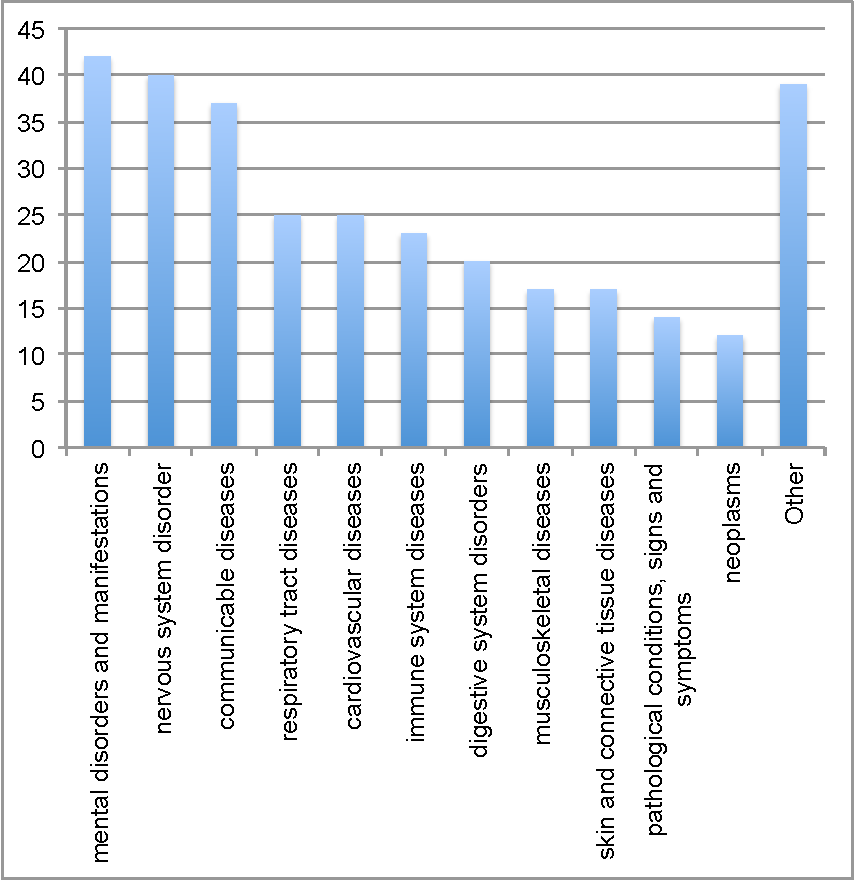
\includegraphics[width=0.9\linewidth]{ch2-figures/Figure3.pdf}
  \end{center}
  \caption[Distribution of indication classes in predicted novel
    usages]{Distribution of indication classes in predicted novel
    usages.  Each indication for the 403 high confidence novel usages
    with support in FAERS and MEDLINE was mapped to the first level of
    the NDF-RT disease hierarchy.  63 usages were not mapped to NDF-RT
    and were left out of this chart.  }
  \label{fig:short}
\end{figure}


\subsection{Plausibility based on mechanisms of action}
We also evaluated the plausibility of the novel, predicted off-label
usages using previously published methods \cite{Sirota2011} applied to
gene expression data from the Connectivity Map \cite{Lamb2006} and
NCBI Gene Expression Omnibus \cite{Edgar2002}.  Briefly, if a drug
modulates gene expression in the opposite manner than a disease
condition, the drug is considered a plausible treatment for the
indication.  This approach requires gene expression data for both drug
exposure and the disease condition.  Of our well-supported novel
usages, two had appropriate publically available data and both yielded
significant gene sets suggesting possible mechanisms of action.  Given
sparse coverage of drugs and diseases in public data, it is difficult
to apply this process systematically.  Nevertheless, this method
yielded testable hypotheses regarding mechanisms of action.  For
instance, simvastatin is linked to diabetes by PPAR-gamma; simvastatin
treatment enriches a gene set known to be activated by PPAR-gamma
activity, while PPAR-gamma agonists, e.g., thiazolinediones, are known
to be used to treat diabetes \cite{Grip2002,Altshuler2000}.

\subsection{Manual validation of the predicted usages}
Examination of the 403 well-supported novel off-label usages revealed
terminological challenges.  For instance, we predict that alendronic
acid is used to treat osteopenia, the clinical precursor to
osteoporosis.  However, Medi-Span and the NDF-RT list the indication
as osteoporosis instead of osteopenia — i.e., they encode the
used-to-prevent relationship. Such issues reflect challenges in
normalizing medical terms.  As a result, although we can detect
used-to-treat relationships quite well, recognizing whether or not
uses are already known is difficult.

Some predicted uses represent bona fide new uses confirmed in the
biomedical literature by case reports, clinical trials, or resources
such as MedlinePlus, but not yet incorporated in our curated sources
of known usage (see Table 2.2 for selected examples).  For instance,
our system predicts that bevacizumab is used to treat ovarian cancer.
This usage has been shown to improve progression free survival in a
phase III trial \cite{Perren2011} and has been approved in the EU, but
does not yet appear in Medi-Span, Drugbank, the NDF-RT or MedlinePlus.
These results show that it is possible to detect emerging off-label
use before it has been officially recognized.


\begin{table}
\begin{center}
\begin{tabular}{|c|c|c|c||}
  \hline Drug Name & Event Name & FAERS & MEDLINE \\ & & Support &
  Support \\ \hline\hline Simvastatin & diabetes mellitus & 1369 & 33
  \\ Tacrolimus & rheumatoid arthritis & 404 & 45 \\ Pregabalin &
  migraine disorders & 152 & 3 \\ Etanercept & lupus erythematosus,
  systemic & 79 & 5 \\ Lamotrigine & migraine disorders & 75 & 6
  \\ Adalimumab & lupus erythematosus, systemic & 71 & 3 \\ Rituximab
  & hodgkin disease & 51 & 48 \\ Daptomycin & osteomyelitis & 45 & 20
  \\ Fludarabine & waldenstrom macroglobulinemia & 39 & 66
  \\ Infliximab & pyoderma gangrenosum & 34 & 68 \\ Erlotinib &
  malignant neoplasm of ovary & 28 & 16 \\ \hline
\end{tabular}
\end{center}
\caption[Selected predicted novel off-label usages]{Selected predicted
  novel off-label usages.  Predicted, novel drug usages with
  substantial support in FAERS.  FAERS Support for each
  drug-indication pair is the number of distinct case reports in FAERS
  in which the drug was explicitly listed as being used to treat the
  indication.  }
\end{table}


\subsection{Prioritizing predicted off-label usages for further investigation}
We designed indices of drug risk and cost using adverse event
associations and unit cost data from Medi-Span to objectively triage
usages for further investigation. The drug risk index is normalized to
lie between 0 and 1, with a value of 0 for drugs with no adverse event
associations in Medi-Span (811 out of 1,602 drugs) and 1 for drugs
associated with many serious adverse events.  Not surprisingly, drugs
with the highest risk indices were immunosupressants, such as
mycophenalate mofetil, and anti-tumor agents, such as gemtuzumab,
clofarabine, bevacizumab, and fludarabine.  Well-supported novel
off-label usages had risk indices ranging from 0.002 for amphotericin
to a maximum of 0.995 for clofarabine.

The drug cost index is based on the mean unit price for the drug in
Medi-Span and is also normalized to lie between 0 and 1, with a value
of 1 for the drug with the highest mean unit cost in Medi-Span.  The
unit cost is an imperfect measure of actual treatment cost — for
instance, it may be for a quantity that is sufficient for multiple
treatments.  Nevertheless, the cost index provides a partial ordering
that is useful for relative ranking because the drugs with the highest
cost index are expensive, targeted therapies such as ranibizumab,
while the drugs with low cost index values are over the counter agents
such as magnesium chloride and iodine.

We used the risk and cost indices to group well-supported novel
off-label usages into high risk, high cost and low risk, low cost
usages, resulting in 28 and 51 usages, respectively (the top 5 usages
in each group are listed in Table 2.3).  We defined thresholds for highs and
lows by looking at the distribution of the risk and cost indices for
the 403 well-supported usages and choosing the upper and lower
quartiles as cutoffs. For example, the upper quartile for the 403
well-supported usages had risk index value 0.828, which defines the
threshold for the high-risk group. For the 403 well-supported usages,
\textbf{Figure 2.1} shows the high–high (28 drug-indication pairs) and
low–low groups (51 drug-indication pairs). Many (16 of 28) of the high
risk, high cost usages involved anti-tumor agents being used to treat
unapproved tumor types. In contrast, the low cost, low risk usages
contain many over the counter drugs such as vitamin E, as would be
expected.

\begin{table}
\begin{center}
\begin{tabular}{|l|l|c|c|c|c||}
  \hline Drug Name & Indication & FAERS & MEDLINE & Risk & Cost \\ & &
  Support & Support & Index & Index \\ \hline\hline
  \multicolumn{6}{|l|}{High risk, high cost usages} \\ \hline
  Docetaxel & Malignant neoplasm & 604 & 640 & 0.964 & 0.949\\ & of
  prostate & & & & \\ \hline Clofarabine & Leukemia, myelocytic,& 341
  & 37 & 0.995 & 0.869 \\ & acute & & & & \\ \hline Rituximab &
  Purpura, & 259 & 169 & 0.940 & 0.821 \\ & thrombocytopenic, & & & &
  \\ & idiopathic & & & & \\ \hline Bevacizumab & Malignant neoplasm &
  170 & 89 & 0.991 & 0.879 \\ & of ovary & & & & \\ \hline Paclitaxel
  & Malignant neoplasm & 122 & 421 & 0.956 & 0.776 \\ & of stomach & &
  & & \\ \\ \hline \multicolumn{6}{|l|}{Low risk, low cost usages}
  \\ \hline Folic acid & mental depression & 493 & 18 & 0.082 & 0.102
  \\ \hline Methadone & depressive disorder & 162 & 33 & 0.002 & 0.167
  \\ \hline Folic acid & hyperlipidemia & 138 & 10 & 0.082 & 0.102
  \\ \hline Megestrol & carcinoma, non-small & 79 & 4 & 0.002 & 0.238
  \\ & cell lung & & & & \\ \hline Folic acid & diarrhea & 67 & 10 &
  0.082 & 0.102 \\ \hline
\end{tabular}
\end{center}
\caption[Ten validated Drug-AEs]{List of ten validated Drug-AEs and
  their support in FAERS as well as MEDLINE}
\end{table}


\section{Discussion}
Off-label usage of drugs is an important enough aspect of drug safety
to warrant a full issue (May 2012) of Nature Clinical Therapeutics and
Pharmacology devoted to the topic \cite{Epstein2012}.  Currently the
most comprehensive information about off-label drug usage is from the
National Disease and Therapeutic Index (IMS Health, Plymouth Meeting,
PA), which relies on periodic surveys of office-based physicians. We
believe that off-label use can be learned systematically, in a
data-driven manner directly from electronic medical records.  Our work
represents the first effort to detect novel off-label usage from
clinical free text over the entire range of drugs and indications
observed in the medical record.  We also developed quantitative risk
and cost indices as a way to prioritize the novel usages for further
investigation.

In the past, NLP has been applied to the problem of detecting
used-to-treat relationships between drugs and indications in clinical
text.  State of the art NLP approaches require training text in which
drug and indication mentions are labeled, along with the relationships
between them.  In contrast, association based approaches that use
counts of drug and indication mentions are more scalable, but limited
by confounding causal and indirect relationships.  We have developed
an automated method for detecting novel off-label usages from clinical
text that does not require training text and addresses confounding
relationships by incorporating prior knowledge about drug usage.  We
applied this method to 1,602 drugs and 1,475 indications to identify
6,142 novel off-label usages, 403 of which are well supported by
evidence in independent and complementary datasets.

Our methods have important limitations.  First, our work focuses on
one form of off-label use — the use of drugs to treat unapproved
indications — and does not detect off-label use with respect to age,
gender, dosage and contraindications.  Second, co-morbidities and drug
adverse events may still lead to spurious used-to-treat relationships
despite our efforts to reduce their impact on our results. Third,
although our method can detect used-to-treat relationships between
drugs and indications with high specificity and good sensitivity, the
task of recognizing whether the knowledge is already known is more
difficult than might be expected.  This difficulty was not due to
errors in recognizing terms in clinical text but rather due to
mismatches in the language used to describe indications in Medi-Span
and the NDF-RT versus clinical text and FAERS.  A systematic listing
of such indication mismatches could identify areas in ontologies and
terminologies that need improvement — and would be a data-driven way
to identify portions of terminologies for review.  Fourth, the risk
and cost indices have some shortcomings.  For instance, the cost index
ignores the fact that dosage and duration of treatment for off-label
usages may differ from approved uses, and our risk index does not take
the dependence of adverse events on dosage, co-morbidities, and
poly-pharmacy into account.  Finally, in this work we have aimed to
produce a list of highly confident predictions of novel off-label
usages so we require corroboration of predictions in FAERS, which has
much lower recall in the test set than the classifier.  Thus the
overall method sacrifices sensitivity for greater specificity.  This
is appropriate for our aim in this work, but other studies may require
a different trade off between sensitivity and specificity.  For
instance, if we were concerned exclusively with potentially risky
usages, we might not require support in FAERS and instead filter for
usages involving drugs associated with known serious side effects that
don’t always get reported.  We note that our method can be modified
for such use cases.

These limitations notwithstanding, our study is the first large-scale
characterization of off-label usage using fully automated methods to
combine information from clinical notes with prior knowledge and to
provide a ranking of the learned usages on risk and cost.  It is a
step towards systematic, data-driven monitoring of off-label usage.
The method has characteristics that allow it to generalize to sites
beyond Stanford.  First, the system does not require training text
labeled with mentions of drugs and indications, and the relationships
between them.  Second, our method is very flexible with respect to the
target drug and indication vocabulary.  Third, the system is very fast
— annotation of 9.5 million clinical notes takes only two hours on a
single machine; constructing features, training a classifier and
making predictions takes an additional few hours.  It is thus
conceivable to process clinical text from a large number of sites,
providing a picture of off-label usage across a wide spectrum of
institutions.

Most importantly, our method was able to detect usages that were
documented in the biomedical literature, and in one case approved in
the EU, despite not appearing in any of our curated sources of known
usage.  This suggests that such systems could potentially provide an
automated learning system for off-label usage.  Such as system could
flag emerging usages before they come to the attention of the broader
medical community, regulatory agencies and drug manufacturers, in much
the same way that Google Flu Trends can provide an early warning of
flu trends in advance of CDC data \cite{Ginsberg2009}.  We speculate
that applying our method to a wider range of clinical text from
multiple sites can provide a timelier and more comprehensive picture
of off-label usage than is currently possible
\cite{Halevy2009,Banko2001}.



\chapter{Learning Adverse Drug Events}
\section{Introduction}
Adverse drug events (ADEs) are undesired harmful effects resulting
from use of a medication. It is estimated that ADEs occur in 30\% of
hospital stays, causing 2 million injuries, hospitalizations, and
deaths each year in the United States at a cost of \$75 billion
\cite{Classen1997,Classen2011,Lazarou1998}. Pre-approval clinical
trials are the first line of defense for identifying adverse drug
events but they are limited both in their power to detect rare events
and their generalizability to patient populations with poly-pharmacy
and many co-morbidities. These limits have driven efforts in
post-marketing surveillance for ADEs using a variety of observational
data sources as a key component of the learning health care system
\cite{Tatonetti2009,Lependu2013,Harpaz2014,Friedman2009}.

These efforts have at their core the collection of counts of drugs
being taken and adverse events occurring, derived from a variety of
data sources. Most work has used spontaneous reporting system data
such as the US Food and Drug Administration’s FDA Adverse Event
Reporting System (FAERS), but other data sources such as claims data
have also been used. Each of these data sources have well-documented
biases. For instance, FAERS relies on voluntary reporting of suspected
drug adverse event cases and suffers from reporting biases such that
associations with adverse events with many possible causes are
difficult to detect \cite{Harpaz2013}, while claims data suffers from
biases arising from its primary use for billing instead of conveying
clinical information \cite{Ryan2013}.

In contrast, the electronic medical record (EMR) and free text of
clinical notes provides arguably the most complete and unbiased
picture of clinical events available \cite{Poissant2010}. There has
been much progress in using methods from Natural Language Processing
(NLP) to extract structured information from the unstructured free
text of clinical notes \cite{Wang2009,Lependu2013}. These studies
typically use Natural Language Processing (NLP) to generate counts of
drug and disorder mentions in the clinical text, often subject to
constraints that reflect, for instance, the intuition that the cause
of an adverse event, e.g., taking a drug, must precede the adverse
event itself. Given such counts, there are two main approaches to
identifying possible drug adverse event associations. One approach,
disproportionality analysis (DPA), tackles the problem using the
well-known framework of statistical hypothesis testing
\cite{Harpaz2013}. These methods use counts of drugs, adverse events,
and their co-occurrence to calculate a p-value for the association of
the drug and adverse event relative to a null hypothesis of no
association, with varying degrees of adjustment for
confounding. However, recent work has shown that using p-values to
prioritize possible drug-adverse event associations is problematic
\cite{Schuemie2014}. Furthermore, it has been noted that integration
of other data sources is likely essential in effective post-marketing
surveillance using observational data \cite{Ryan2013}. However, it is
not clear how to effectively incorporate some forms of relevant
information, such as prior knowledge of known ADEs. Such prior
knowledge may be especially helpful for detection of ADEs in which the
drug or adverse event is rare.

An alternative to statistical hypothesis testing is using
discriminative classifiers such as a logistic regression model. These
methods differ from DPA in that they attempt to learn a function that
guesses the validity of drug adverse event associations given inputs,
or features, such as counts of the drug and the adverse event in the
data. Importantly, the input can include features that reflect prior
knowledge such as similarity to known adverse drug events. Such
discriminative classifiers can be applied to spontaneous reports or to
EMR derived counts. Harpaz et al \cite{Harpaz2013} conducted a
systematic review of drug adverse event algorithms using FAERS data
that found logistic regression methods outperforming state of
the art DPA methods across a variety of adverse events. Recent work by
Noren et al has shown that building such a discriminative classifier
that uses additional information such as the geographic origin of an
adverse event report and the timing of the submission achieves much
better performance than existing methods
\cite{Caster2014,Caster2013,Harpaz2013b}. Cami et al \cite{Cami2011}
went even further and developed a logistic regression model using only
features encoding prior knowledge about known ADEs that achieved high
performance.  Liu et al \cite{Li2011} used a discriminative classifier
to distinguish adverse drug events (pairs of drugs and adverse events
in which the drug causes the adverse event) from drug usages (pairs of
drugs and disorders in which the drug is used to treat the
disorder). Their classifier used features derived from the free text
of millions of clinical notes from the Stanford Translational Research
Integrated Database Environment (STRIDE) \cite{Lowe2009} that encoded
the frequency of drug and disorder mentions and co-mentions in the
text, subject to constraints on the order of the mentions in
time. However, this preliminary work simply evaluated the performance
of the classifier using cross validation and did not attempt to
discover novel drug adverse event associations. It also restricted
itself to drug-disorder pairs in which both the drug and disorder were
frequently mentioned together, limiting its utility for detecting rare
AEs. In related work, Jung et al \cite{Jung2014} used EMR derived
features to detect drug usage pairs, but also added additional
features encoding prior knowledge about known drug usages. These
additional features were found to significantly improve the
performance of the classifier in a validation set, and the classifier
was applied to all possible drug and indication pairs to identify
putative off-label drug usages.

We have built on this work, developing a method suited for systematic,
automated detection of potential adverse drug events from the EMR. Our
method uses the text from clinical notes, along with prior knowledge
of drug usages and known adverse drug events, as inputs. We use a
computationally efficient text processing system to extract mentions
of drugs and disorders from the text. These mentions are further
processed into statistics that are used by a discriminative classifier
that outputs the probability that a given drug-disorder pair
represents a valid adverse drug event association. The classifier
achieved an area under the ROC curve (AUC) of 0.94 on hold out test
data. Applying it to all possible drug-adverse event pairs and
filtering the predicted ADEs support in independent and complementary
data sources – FAERS and MEDLINE – resulted in 240 high-confidence
ADEs. Figure 3.1 summarizes our approach.

\begin{figure}
  \begin{center}
    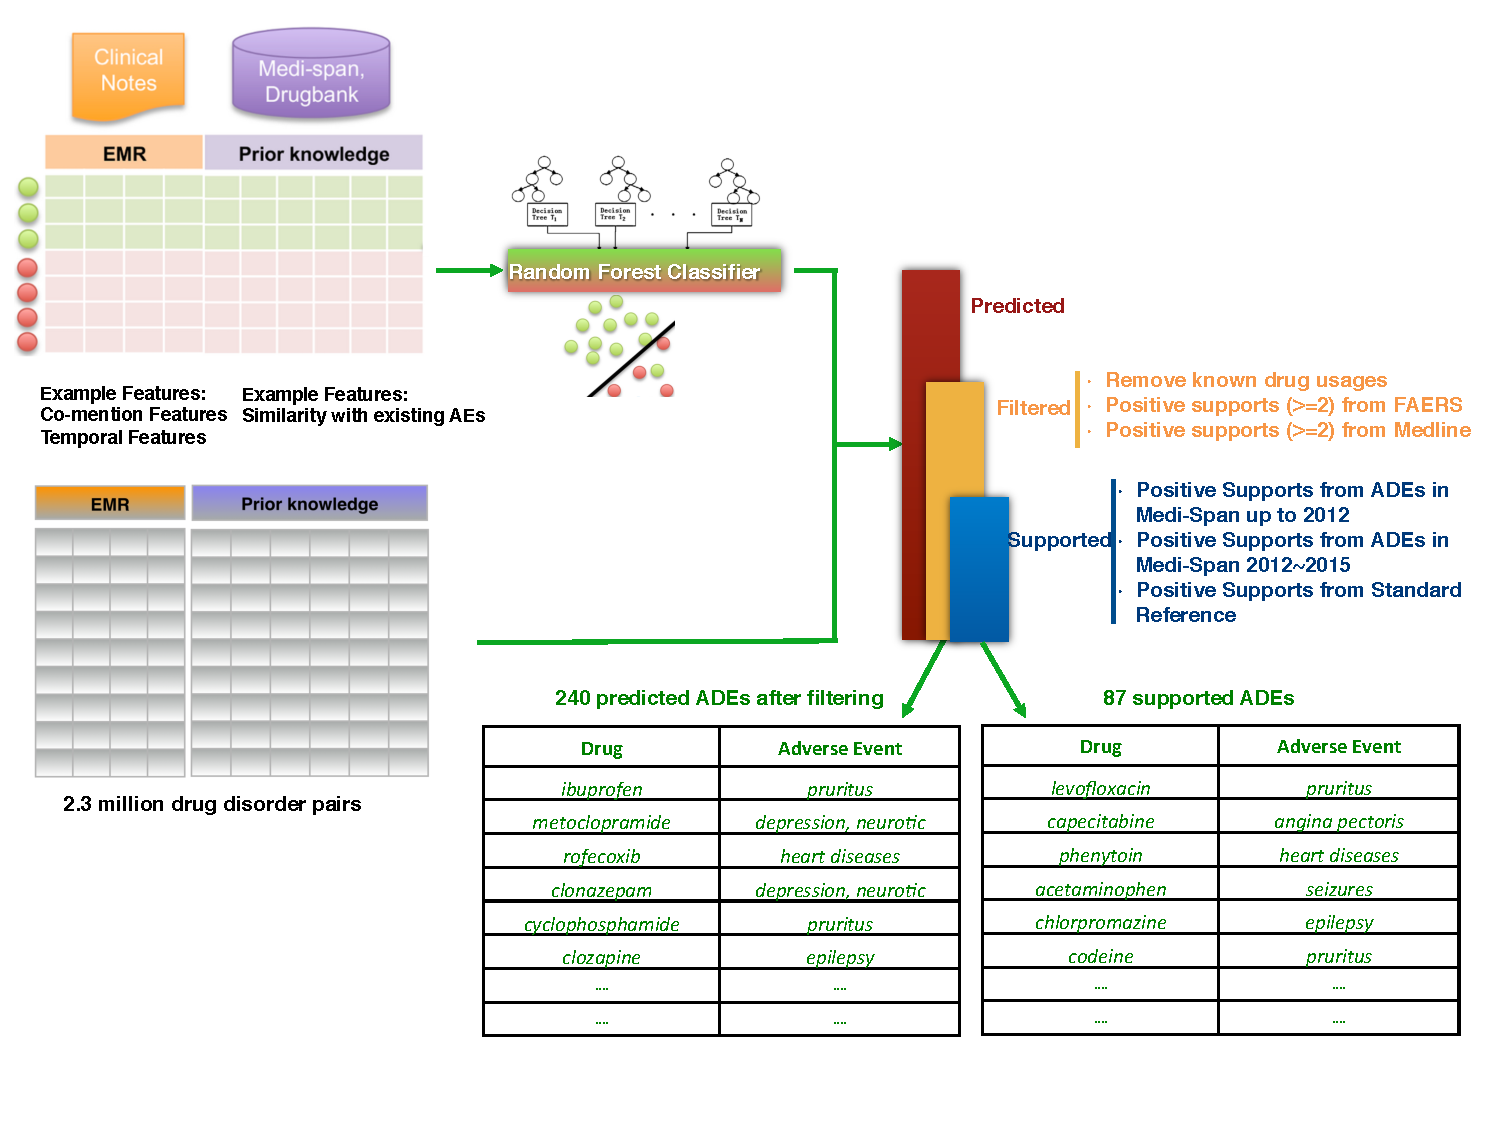
\includegraphics[width=0.9\linewidth]{ch3-figures/Figure1.pdf}
  \end{center}
  \caption[Feature engineeering for ADE discovery]{For each of the
    2,362,950 possible drug-disorder pairs, we calculated 9 features
    from the free text of clinical notes in STRIDE, 8 features from
    known AEs in Medi-Span, and 12 features from known usages in
    Medi-Span and Drugbank. Based on these features, a Random Forest
    classifier was trained on the gold standard dataset to recognize
    the drug-AE relationships. Then, we applied the trained
    classifiers to the possible drug-disorder pairs and
    filtered for support in FAERS and MEDLINE, yielding a set of 240
    predicted ADEs. Drug-AE pairs used in training are also removed.  }
  \label{fig:short}
\end{figure}


\section{Materials and Methods}
\subsection{Constructing training and test sets}
Discriminative classifiers learn a function that maps input features
to an output such as the probability that the inputs represent a true
drug adverse event pair. In order to learn and evaluate the
performance of this function, these methods require a set of examples
of drug adverse event pairs whose status as true or false associations
is known. We constructed such a set of positive and negative examples
of drug-AE pairs using known ADEs from Medi-Span® Adverse Drug Effects
Database (from Wolters Kluwer Health, Indianapolis, IN). Medi-Span up
to 2012 contains 711,468 drug-disorder pairs comprising 13,000 unique
drugs and 3,403 unique disorders. Of these, 3,550 pairs were assumed
to be true adverse drug event pairs because they occur in black box
warnings with additional constraints (e.g. above moderate severity
level). We used RxNorm to normalize drugs to their active ingredients
and discarded pairs in which either the drug or adverse event did not
occur in the EMR data. This resulted in 1,898 positive examples for
training and testing. To construct negative examples, we randomly
sampled drugs and adverse events from among the drugs and adverse
events in the positive set and ensured that the co-mention counts
distribution of the negative samples are roughly the same as those of
the positive samples. 4,336 such negative samples remained after
removing inadvertently generated positive examples. These drug adverse
event pairs were then randomly split into 4,358 training examples used
to learn classifiers and 1,877 test examples used to evaluate the
performance of the classifiers.

\subsection{Processing of clinical text-notes from STRIDE}
An NCBO Annotator based text-processing pipeline
\cite{Lependu2012,Jung2014b} was used to annotate 9.5 million clinical
notes from STRIDE with mentions of drugs and disorders. Negated
mentions (e.g., “MI was ruled out”) or those referring to other people
(e.g., “father had a stroke”) were removed using NegEx
\cite{Chapman2001} and ConText \cite{Chapman2007}, respectively.  The
notes spanned 18 years and 1.6 million patients. Drugs and disorders
were mapped to UMLS unique concept identifiers (CUIs). In this study
we used the 2011AB version of the UMLS. Drugs were normalized to
active ingredients using RxNorm \cite{Nelson2011} as provided by
UMLS2011AB – for example, Panocaps was normalized to lipase, protease,
and amylase.

\subsection{Feature construction}
For each drug-disorder pair, we constructed nine features from the
clinical note derived mentions – the drug and disorder frequency,
co-mention frequency, drug first fraction (the fraction of patients in
which the first mention of the drug precedes the first mention of the
disorder) and association scores derived from these counts (e.g., chi
squared statistic, odds ratio, and the conditional probability of drug
mention given disorder mention).

In addition, we constructed eight features encoding known drug-AEs and
twelve features encoding known usages. Those features were motivated
by the intuition that a drug may be more likely to cause an adverse
event if similar drugs are known to cause that adverse event. Known
AEs were defined as appearing in Medi-Span. For each drug-disorder
pair, we computed the similarity of the drug to drugs known to cause
the disorder, and the similarity of the disorder to other disorders
caused by the drug. The calculation of drug-drug and disorder-disorder
similarity is described in Figure 3.2. For usage-similarity, we
adopted features described in Jung et al \cite{Jung2014}. In all, we
used 29 features for each drug-disorder pair.

\begin{figure}
  \begin{center}
    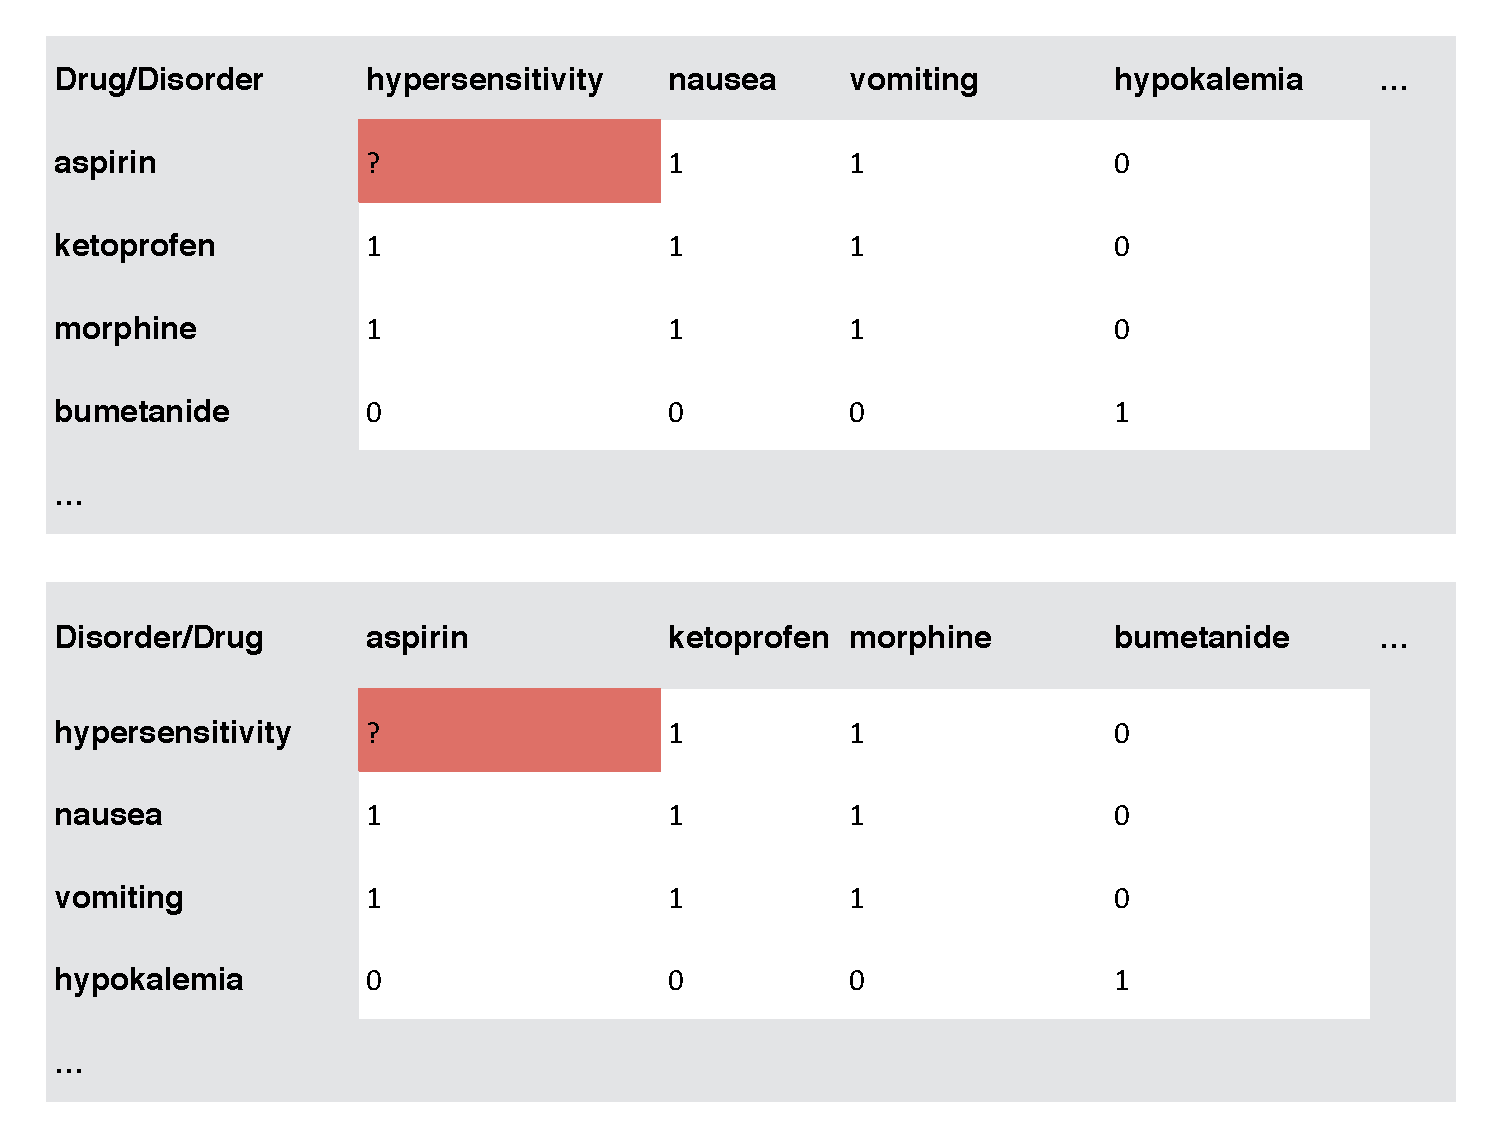
\includegraphics[width=0.9\linewidth]{ch3-figures/Figure2.pdf}
  \end{center}
  \caption[Calculating drug-drug and disorder-disorder similarity]{
    We represent prior knowledge about ADEs as matrices in which each row is a
    drug and each column is an AE.  The (i,j)-th entry is an indicator
    for whether or not the drug i is known to be associated with AE
    j.  We are interested in computing a feature that captures the
    intuition that drugs with similar adverse event profiles are more
    likely to also be associated with a new, unknown adverse event.
    Say we are interested in the associationn of drug i with AE j.  We
    first find other drugs which are \emph{known} to be associated
    with AE j.  We then compute the similarity of drug i with all of
    these drugs using cosine and Jacquard similarity.  These
    similarities are then pooled over the set of other drugs by using
    the max and the mean.  To calculate drug-drug similarity with
    respect to other characteristics such as targeted molecular
    pathways from Drugbank, we simply use a matrix in which the
    columns represent pathways.  To calculate disorder-disorder
    similarity, we perform an analogous calculation with the roles of
    drugs and AEs reversed.}
  \label{fig:short}
\end{figure}


\subsection{Classifier development}
We fit L1 regularized logistic regression (lasso) \cite{Lasso}, SVM
with radial basis function kernel \cite{SVM} , and random forest
classifiers \cite{Liaw2002} to the training data. Model
hyperparameters were fit by cross validation in the training data.
The classifiers were then evaluated on the hold out test set. The
classifier development process is summarized in Figure 3.3. In order
to investigate the contribution of different features, we performed an
ablation analysis in which we evaluated classifiers using subsets of
the features.

\begin{figure}
  \begin{center}
    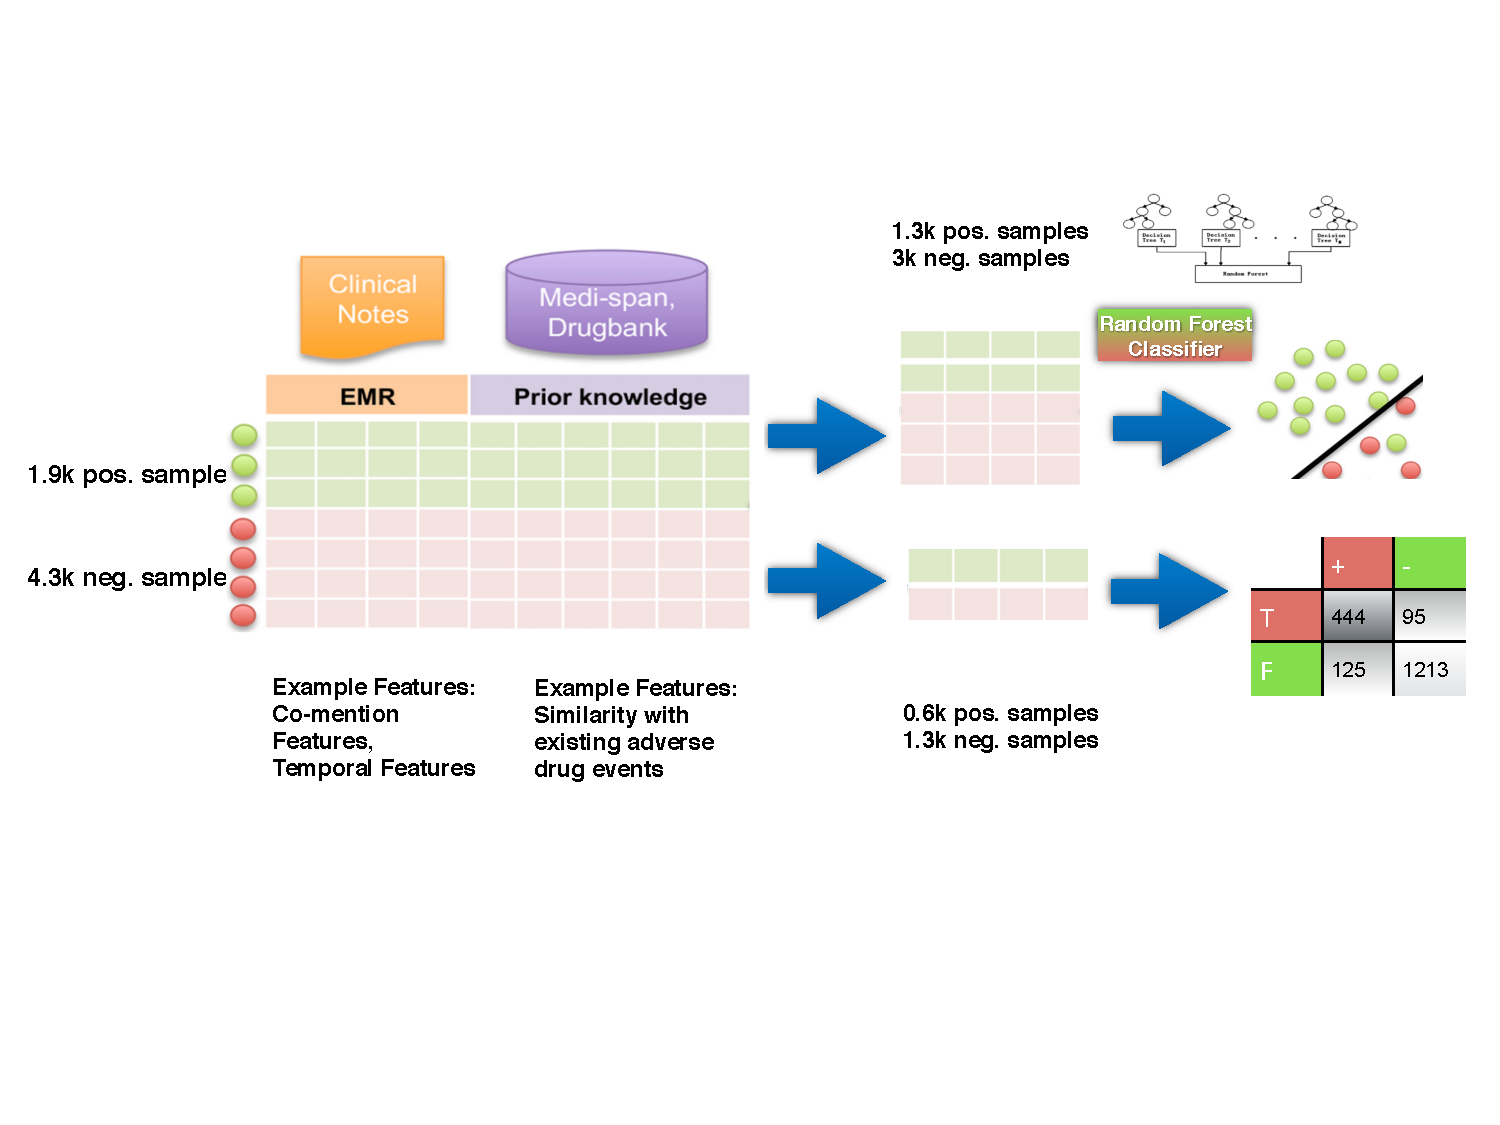
\includegraphics[width=0.9\linewidth]{ch3-figures/Figure3.pdf}
  \end{center}
  \caption[Training a classifier to recognize ADEs]{Positive examples
    collected from known drug AEs in Medi-Span and negative examples
    created through randomly sampling a drug and disorder with roughly
    the same co-mention distribution as the positive examples. For
    each drug-disorder pair in the gold standard, we used 9 features
    to characterize the pattern of drug and disorder mentions in 9.5
    million clinical notes from STRIDE, 8 features to characterize the
    domain knowledge of drug, disorder, and known AEs from Medi-Span,
    and 12 features to characterize the domain knowledge of drug,
    disorder, and known usages from Medi-Span and Drugbank. The gold
    standard dataset was randomly split into 70\% for training and
    30\% for testing the classifier.}
  \label{fig:short}
\end{figure}


\subsection{Identifying putative drug-AE associations}
Performance on the test set indicated that the random forest
classifier was superior to the other classifiers in all metrics. We
therefore focused on this model and applied a classifier trained on
the full gold standard dataset to the 2,362,950 possible drug-AE pairs
comprised of 1,602 unique drugs and 1,472 unique disorders appearing
in our data. We focused on the most confident predicted associations
by using a threshold of 0.7 for the posterior probability output by
the classifier, yielding 41,248 predicted ADE associations.  Known
ADEs and drug usages were then filtered out.  In this study, the set
of 3,550 known ADEs were gathered from the Medi-Span® Adverse Drug
Effects Database, where the documentation level is marked as “black
box warning”; known usages were gathered from the Medi-Span Drug
Indications Database (Wolters Kluwer Health, Indianapolis, IN) and the
National Drug File – Reference Terminology (NDF-RT) \cite{Brown2004}.

\subsection{Filtering in FAERS and MEDLINE}
We filtered the drug-AE associations using FAERS \textbf{REF} and
MEDLINE, two independent and complementary data sources that reflect
clinical practice and published biomedical knowledge
respectively. FAERS case reports contain explicit links between drugs
and adverse events. We used all case reports from Q1 2005 through Q4
2013 to assess support for putative ADEs in terms of the number of
case reports in which the drug was reported as the primary or
secondary suspect drug for the adverse event. FAERS drugs and adverse
events were mapped to UMLS CUIs, yielding a set of 4,508,892
drug-event reports covering 372,379 unique pairs. We also obtained
reports of adverse drug events described in the biomedical literature
from MEDLINE. Using an approach described by Winnenburg et al
\cite{Winnenburg2015}, we obtained 118,552 unique ADEs from about
200,000 articles in MEDLINE that had been manually annotated with
combinations of Medical Subject Heading (MeSH) descriptors and
qualifiers for both a drug involved in an adverse event (e.g.,
Ofloxacin/adverse effects) and its manifestation (e.g.,
Tendinopathy/chemically induced). We mapped the MeSH terms of drug -
disease pairs (e.g., Ofloxacin – Tendinopathy) to their corresponding
UMLS CUIs to make the findings compatible with our predictions.

\subsection{Validation in Medi-Span and Time-Indexed Reference}
We validated the drug-AE associations using future years of data from
Medi-Span. The training examples used in our model were constructed
from ADEs marked as “black box warning” in Medi-Span up to 2012—thus
we only used well-established adverse events in training the
classifier. Medi-Span also contains ADEs marked as “reported in
multiple reports and uncontrolled studies” or “reported in few case
reports and suggested links”; we refer to these ADEs with moderate
support.  We validated the drug-AE associations left after filtering
based on FAERS and MEDLINE using ADEs with moderate support in both
Medi-Span up to 2012 as well as with the additional Medi-Span data
from 2012 to 2015.  Medi-Span up to 2012 contains 95,115 ADEs with
moderate support, and Medi-Span from 2012 to 2015 contains an
additional 755 ADEs that were not reported in Medi-Span as of 2012. In
addition, we used a time-indexed reference standard by Harpaz, R. et
al. \cite{Harpaz2013b} to further assess the classifier’s ability to
detect recent drug-AE associations. The reference standard was
systematically curated from drug labeling revisions (e.g. new warnings
issued and communicated by the US Food and Drug Administration in
2013), and included 62 positive test cases and 75 negative controls.

\subsection{Feature contribution}
We performed feature ablation experiments to investigate whether or
not our encoding of domain knowledge contributed to model
performance.  We grouped the twenty-nine features into
three categories: features from Clinical Notes (CN), features from
known AEs (KA), and features from known usages (KU).  Classifiers were
trained on each of these subsets of features, along with the
combinations CN+KA and CN+KU.  The performance of these models were
then evaluated on the test set. 

\section{Results}
\subsection{Performance of the classifier}
The random forest classifier to detect drug-AE associations achieved
an AUC of 0.94 in a hold out test set. We then fit a new random forest
classifier using the entire gold standard and applied it to the
2,362,950 drug-AE pairs arising from 1,602 unique drugs and 1,472
unique disorders appearing in our data. After applying a cutoff on the
classifier’s confidence (posterior probability of 0.7), we arrived at
a set of 41,248 putative drug-AE associations. We refined these 41,248
drug-AE associations by filtering for support in FAERS and
MEDLINE. 240 associations were supported by at least 2 reports in both
FAERS and MEDLINE. Table 3.1 lists the ten associations with the
highest level of support in FAERS.

\begin{table}
\begin{center}
\begin{tabular}{|c|c|c|c|c|c||}
  \hline Drug Name & Drug CUI & Event Name & Event CUI & FAERS &
  MEDLINE \\ & & & & Support & Support \\ \hline\hline etanercept &
  C0717758 & pruritus & C0033774 & 11485 & 2 \\ metoclopramide &
  C0025853 & depression, neurotic & C0282126 & 1473 & 9 \\ rofecoxib &
  C0762662 & heart diseases & C0018799 & 861 & 3 \\ clonazepam &
  C0009011 & depression, neurotic & C0282126 & 691 & 2 \\ diazepam &
  C0012010 & depression, neurotic & C0282126 & 608 & 5 \\ levofloxacin
  & C0282386 & pruritus & C0033774 & 540 & 3 \\ cyclosporine &
  C0010592 & pruritus & C0033774 & 517 & 5 \\ clozapine & C0009079 &
  epilepsy & C0014544 & 410 & 13 \\ lorazepam & C0024002 & depression,
  neurotic & C0282126 & 403 & 3 \\ ibuprofen & C0020740 & pruritus &
  C0033774 & 374 & 4 \\ \hline
\end{tabular}
\end{center}
\caption[Ten validated ADEs and their support in FAERS and
  MEDLINE]{List of ten validated Drug-AEs and their support in FAERS
  as well as MEDLINE}
\end{table}

\subsection{Contribution of feature sets}
We evaluated the performance of models trained on subsets of the
features to investigate their contribution to model performance.  The
results are summarized in Table 3.2.  Classifiers using features from
clinical notes, known AEs, and known usages had AUCs of 0.92, 0.72 and
0.82 respectively. Classifiers that used both clinical note features
and known ADE or usage information achieved an AUC of 0.93. Above the
features derived from clinical notes, features from prior knowledge
contributed little in our classifier. Thus, it may be helpful to
incorporate the features used in Cami et al’s in the model. Adding
features from known AEs or known usages to features from clinical
notes significantly improved the classifier performance in terms of
sensitivity, while all features together resulted in a sensitivity of
0.839 and an AUC of 0.944.

\begin{table}
\begin{center}
\begin{tabular}{|c|c|c|c|c||}
  \hline Feature set & AUC & PPV & Specificity & Recall
  \\ \hline\hline Clinical Notes (CN) & 0.920 & 0.763 & 0.803 & 0.702
  \\ Known Adverse-Event (KA) & 0.723 & 0.526 & 0.624 & 0.550 \\ Know
  Usage (KU) & 0.815 & 0.561 & 0.661 & 0.584 \\ CN+KA & 0.932 & 0.775
  & 0.714 & 0.801 \\ CN+KU & 0.937 & 0.781 & 0.719 & 0.820 \\ ALL &
  0.944 & 0.796 & 0.913 & 0.839 \\ \hline
\end{tabular}
\end{center}
\caption[Performance of ADE classifier]{Performance of Random Forest
  classifier on held-out test set with different feature sets}
\end{table}


\subsection{Assessing the quality of the predictions}
Out of the 240 well-supported drug-AE associations, 76 occurred in the
set of the ADEs with moderate support in Medi-Span up to 2012. We also
found that 10 out of the 240 drug-AE associations occurred in the
recent established ADEs included in the additional Medi-Span data from
2012 to 2015. Finally, two of the drug-AE associations were also
supported by the reference standard provided by Harpaz, R. et al.
Figure 3.4 shows the support from those data sources for the predicted
drug-AE associations. Overall, from the 240 drug-AE associations, 87
of them (36\%) are supported in at least one of the resources that
have information not available to the classifier.

\begin{figure}
  \begin{center}
    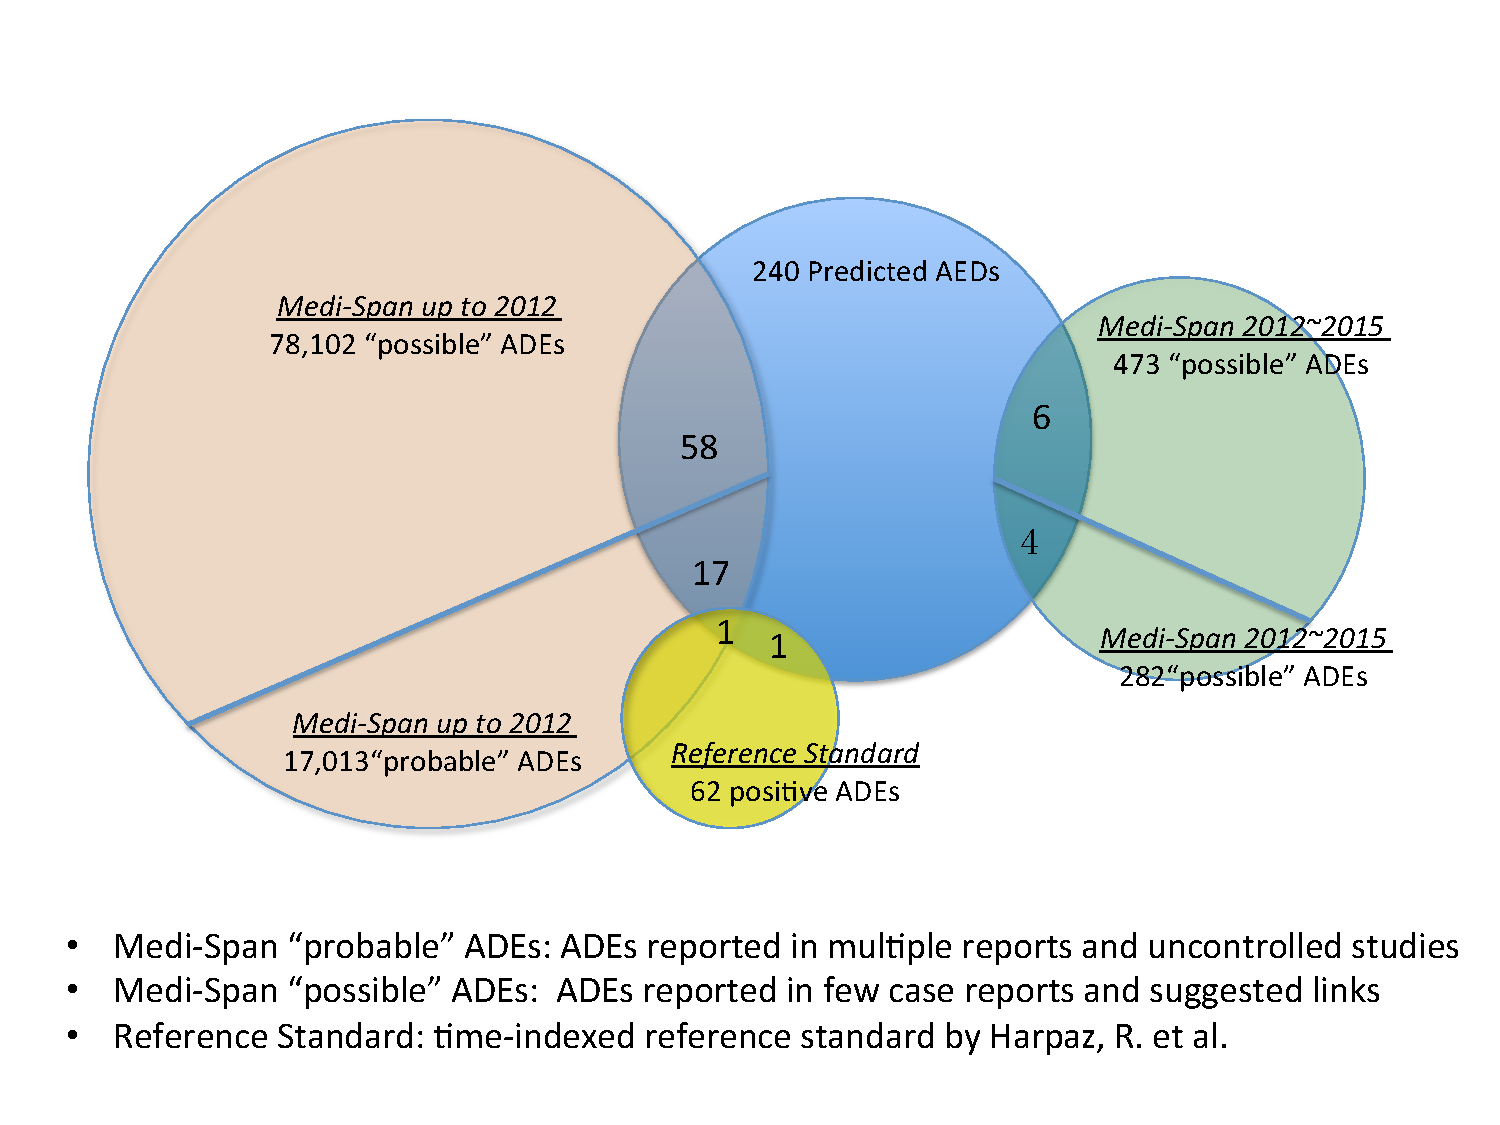
\includegraphics[width=0.9\linewidth]{ch3-figures/Figure4.pdf}
  \end{center}
  \caption[Validation of predicted ADEs]{We validated the predicted
    drug-AE associations from three independent and complementary data
    sources. From the 240 drug-AE associations, 76 occurred in the set
    of the ADEs with moderate support in Medi-Span up to 2012; 10
    occurred in the recent established ADEs included in the additional
    Medi-Span data from 2012 to 2015; two occurred in the reference
    standard provided by Harpaz, R. et al. Overall, 87 of them (36\%)
    were supported in at least one of the resources which have
    information that was not available to the classifier.  }
  \label{fig:short}
\end{figure}


\section{Discussion}
We have developed a method for systematic, automated detection of
adverse drug events. The method achieves high specificity and
sensitivity in a hold out test set using features derived from both
clinical notes and prior knowledge about drug usages and adverse drug
events. Our classifier does not make any assumptions on relationship
between the inputs, allowing us to easily incorporate disparate types
of knowledge into the predictions. In particular, features derived
from clinical notes are empirical, and reflect clinical practice as
is, while features encoding prior knowledge potentially allow us to
make better predictions in cases where the empirical data is lacking.
The direct use of EMRs also opens the door to prioritizing potential
novel ADEs using the observed frequency of co-occurrence of the drug
and adverse event in the EMR, which may better reflect their true
prevalence than data sources such as FAERS. We note that systematic
detection of adverse drug events requires methods that are easily
applicable to many health care institutions. Our method has several
characteristics that make it especially suitable for such use. First,
its input is primarily derived from clinical free text through a
computationally efficient text processing system that can handle
millions of notes in hours. Second, unlike other approaches to
enabling cross institution analysis of EMR data, our method assumes
only access to the text of clinical notes without assuming a common
data model. Third, it is easy to adapt the classifier to different
institutions because no components other than the classifier need site
specific tuning. The latter is not an obstacle to adoption because the
training and validation of the classifier can be entirely
automated. These characteristics of our approach minimize the
computational and organizational demands of implementing the method in
a variety of settings.  Our work has important limitations. First, we
emphasize that the classifier generates hypotheses (i.e. “signals” of
a putative association) instead of verified ADEs. Furthermore, our
working definition of novelty in this study is novelty with respect to
a set of well-established ADEs. We view this positively, as further
validation of our method, because our primary aim is to demonstrate
the feasibility of an approach to post-marketing surveillance which is
suitable for large scale deployment across many health care
institutions. We note that in practice, the set of ‘known ADEs’ used
in training could be tuned to change the sensitivity of the
classifier. We also note that despite the classifier’s high
specificity in test data, applying it to millions of hypothetical
drug-AE pairs may result in a large absolute number of false
positives. Second, as in previous studies that have used free text to
discover relationships between drugs and disorders, the mismatch
between terms as they are formally defined in formal ontologies versus
how they are used in practice may lead to seemingly novel results that
in fact already known \cite{Jung2014}. Third, we note that while the
use of clinical notes may provide an estimate of prevalence that can
be used to prioritize findings for further study, it would be better
still to combine prevalence with severity, which may require deeper
natural language processing to ascertain severity. Finally, we note
that any biases that are present in the training set of known ADEs
will likely carry over to predictions made on a wider range of drug
adverse event pairs, potentially leading to missed
associations. Furthermore, with respect to the use of this method for
systematic, nation-wide post-marketing surveillance, we note that the
problem of optimally integrating safety signals from multiple sites is
an unsolved research problem despite recent progress
\cite{Harpaz2013c}. Meta-analysis approaches of weighted voting
schemes are necessary to combine the signals generated by such a
classifier from multiple sites.  Despite these limitations, this
method is an important first step towards automated, systematic and
comprehensive post-marketing surveillance for ADEs using electronic
medical records as the primary source; such ability is an important
use case envisioned for the learning health care system [10]. We
envision a future in which it is possible to generate hypotheses of
adverse drug events automatically, in real time, and queue them up for
potential review and submission to the Federal Adverse Event Reporting
System.

\section{Conclusion}
We have developed and validated a data-mining method for identifying
putative, new adverse drug events using clinical data and prior
knowledge of known ADEs. Our classifier achieves high discrimination
capability with an AUC of 0.94 on a held out test set. By applying the
classifier to 2,362,950 drug-disorder pairs consisting of 1,602 unique
drugs and 1,472 unique disorders we identified 240 high-confidence
drug-AE associations. These high-confidence associations are well
supported by multiple independent and complementary resources. Our
method enables systematic post-marketing surveillance for new ADEs
using EMRs.



\chapter{Functional evaluation of text-mining tools}
\section{Introduction}
Clinical text from Electronic Health Records (EHRs) has been used for
post-marketing surveillance of drug-induced adverse events
\cite{Harpaz2010,Haerian2012,Wang2009,Friedman2009,Liu2013,Platt2012},
detection of drug-drug interactions \cite{Iyer2013,Duke2012},
discovery and validation of clinical phenotypes
\cite{Lyalina2013,Pathak2013,Davis2013}, and detection of
relationships between clinical concepts, such as drug-disease
treatment pairs
\cite{Jung2014,Chen2008,Zhu2013,deBruijn2011,Patrick2010}.  Raw
clinical text arguably provides the most complete picture of the state
of patients at any point in time since much of the structured data in
EHRs, such as administrative codes, are used primarily for purposes
other than communication of key clinical information about patients –
e.g., billing \cite{Poissant2010,BirmanDeych2005,Carroll2012,Xu2013}.
However, clinical text is unstructured data, and basic questions that
are easy to state in plain language are often difficult to reduce to
practice – for example, find all patients who have Peripheral Artery
Disease and who are taking Cilostazol.  A critical first step in the
use of clinical text to address such electronic phenotyping problems
is finding mentions of entities of interest, such as drugs, diseases
or laboratory values in the text \cite{Boland2013,Bauer2013}.  These
may be positive mentions, indicating that the patient has the disease
or is taking the drug, or negated mentions, such as when a condition
is ruled out.  These mentions may then be used to calculate statistics
to directly address the question at hand, or as the basis for
representing patients for use in data mining approaches
\cite{Boland2013,Bauer2013,Cole2013}.

A variety of Natural Language Processing (NLP) systems that address
this goal have already been developed and are in widespread use
\cite{Chen2004,Davolio2010,Savova2010}.  These may be arranged along a
spectrum of complexity, from very simple, fast string matching systems
to more complex systems incorporating sophisticated statistical
learning methods \cite{Nadkarni2011,Deshmukh2009,Meystre2010}.
Simpler systems typically provide a minimal set of information about
the text, such as mentions of entities of interest and their negation
status.  More complex systems often provide much richer information
about the text, such as part of speech tags and parse trees, in
addition to mentions of entities of interest.  However, this comes at
a significant cost in the form of increased computational demands and,
in the case of supervised learning methods, the need for labeled
training text from which to learn.

In this paper, we present a systematic exploration of the tradeoffs
between simple term recognition and advanced NLP methods when applied
to clinical text for a diverse set of use cases.  We used a modified,
standalone workflow based on the NCBO Annotator
\cite{Noy2009,Lependu2012b,Jonquet2010} and REVEAL (Health Fidelity,
Palo Alto CA), to find mentions of entities of interest in 9 million
clinical notes from the Stanford Translational Research Integrated
Database Environment (STRIDE) \cite{Lowe2009}, and investigated
tradeoffs between these two sets of term-mentions when they were used
in several clinical research tasks (Figure 4.1).

\begin{figure}
  \begin{center}
    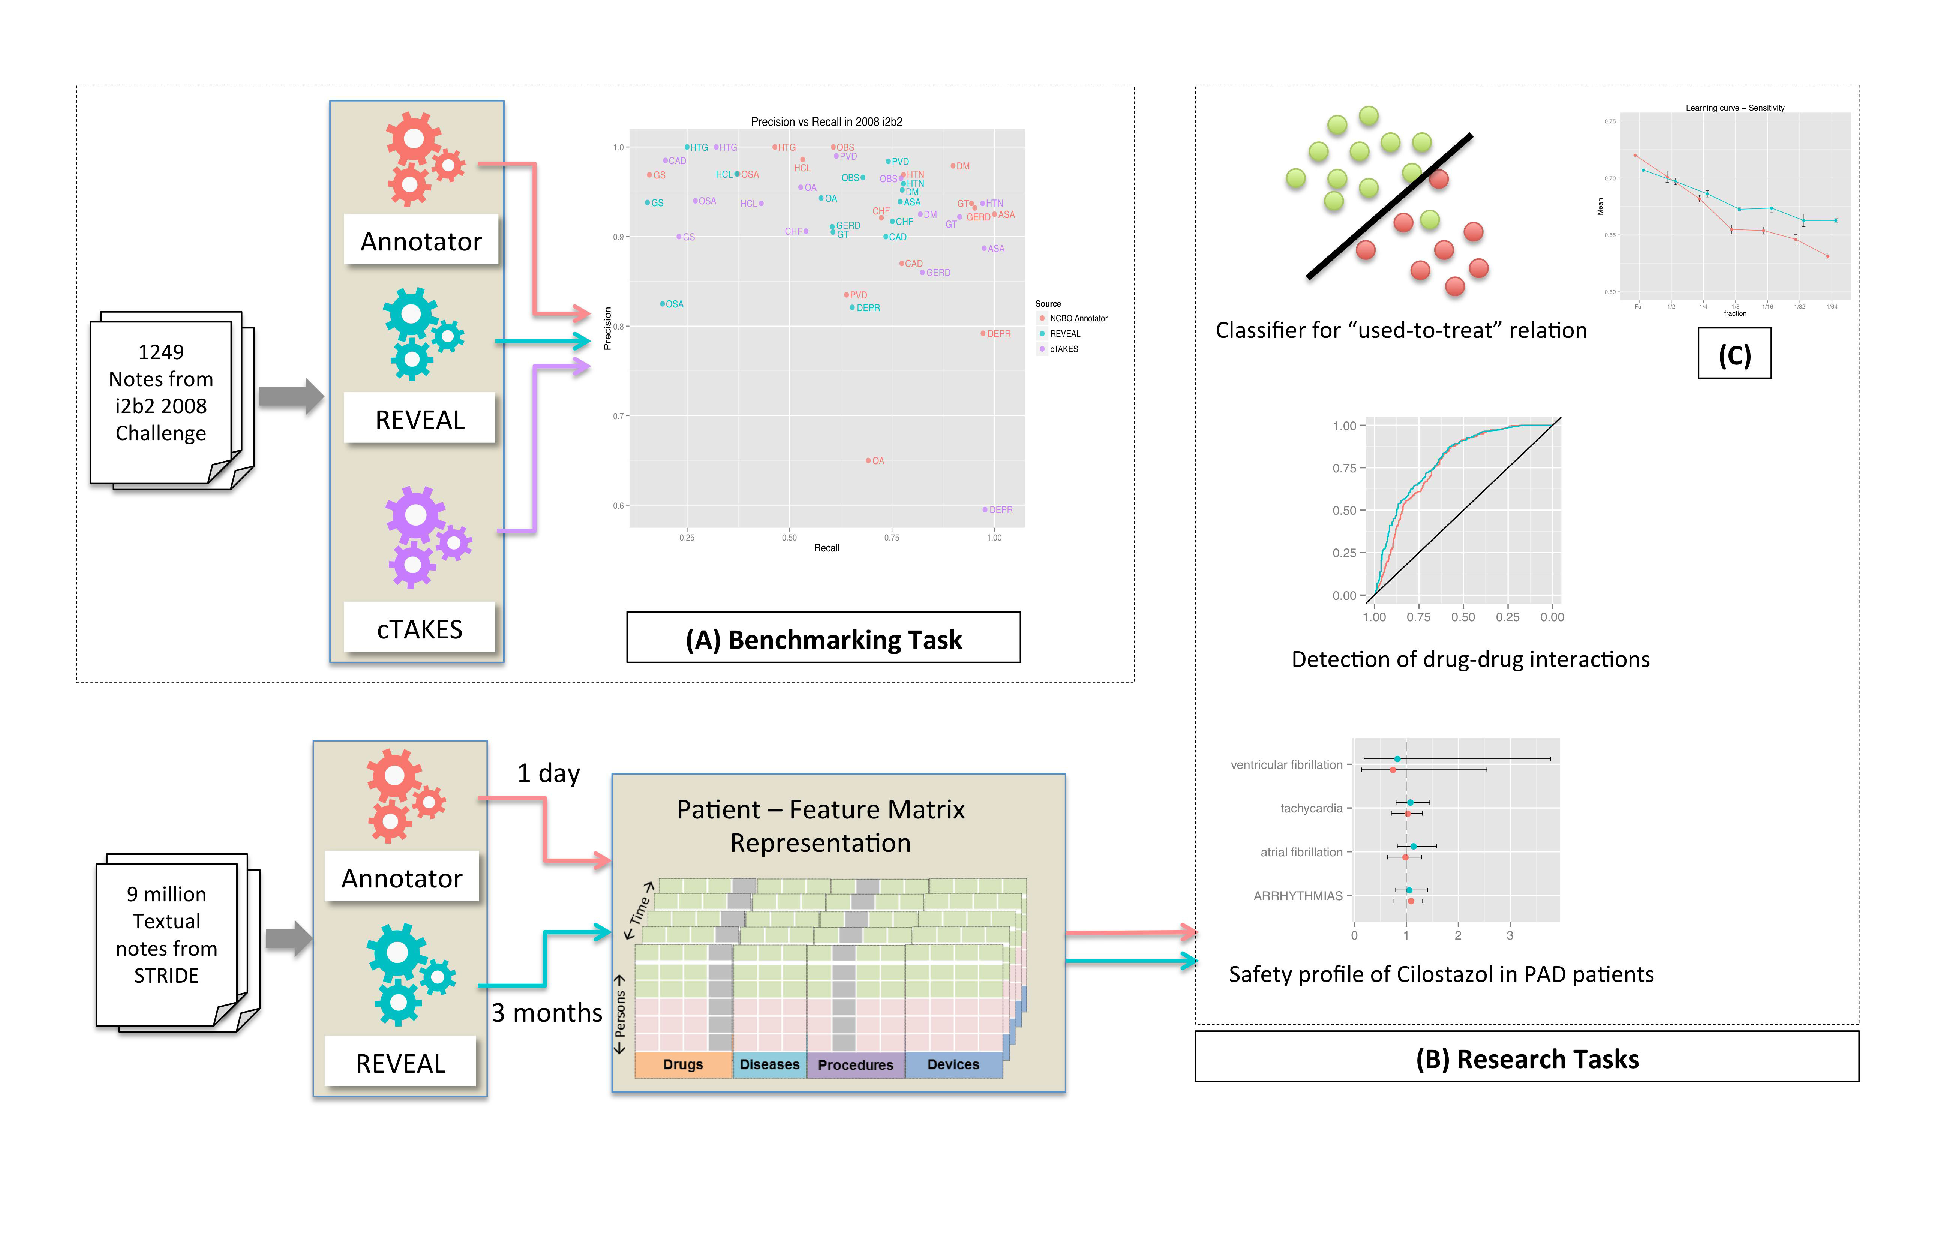
\includegraphics[width=0.9\linewidth]{ch4-figures/Figure1.pdf}
  \end{center}
  \caption[Overview of text processing tool comparison]{Our
    investigation has three parts: (A) First, we benchmark the
    accuracy of the NCBO Annotator based workflow, REVEAL and cTAKES
    on the task of finding mentions of co-morbidities in the 2008 i2b2
    Obesity Challenge dataset (details in Figure 4.2). (B) Second, we
    evaluate the trade-off of using annotations, and the resulting
    patient-feature matrix, from 9 million clinical notes from STRIDE
    generated using the NCBO Annotator based workflow and the REVEAL
    NLP system. The three research tasks are: detection of
    used-to-treat relationships between drugs and indications,
    detection of drug-drug interactions and profiling the safety of
    Cilostazol use in patients with Peripheral Artery Disease. Each of
    these evaluations is based on previously published work; the only
    source of variation is the annotations used as input to the
    published methods. The patient-feature matrix is described in
    detail in Supplemental materials S2. We did not run cTAKES on the
    9 million clinical notes from STRIDE because it would have
    required over a year to complete given our computational
    resources. (C) Finally, we explore the impact of dataset size on
    task of detecting the used-to-treat relation using increasingly
    smaller subsets of the data (details in figure 6).}
  \label{fig:short}
\end{figure}


The NCBO Annotator based workflow is a minimalist system that relies
on a large dictionary of terms, their mappings to UMLS concept IDs
(CUI’s) \cite{Bodenreider2004}, and the NegEx negation detection
system \cite{Chapman2001}, to find mentions of biomedical concepts in
clinical text and establish their negation status.  There is little
“understanding” of the text aside from recognizing a set of words and
phrases, and their negations.  The workflow is deployed quite
directly, using computationally efficient string matching and regular
expression engines \cite{Shah2009,Unitex} that operate directly on the
text without any pre-processing.  In contrast, REVEAL, a commercial
NLP system based on the popular MedLEE system \cite{Friedman2000},
performs various pre-processing steps such as parsing and word sense
disambiguation en route to encoding words and phrases into UMLS codes.
These steps represent a deeper understanding of the structure of the
text than that of the NCBO Annotator based workflow, and are expected
to improve the quality of the annotations.

However, it took roughly 3 months to process our dataset with REVEAL,
while the NCBO Annotator processed the same dataset in a few hours.
It is thus worth exploring what is gained from this extra
computational time when we employ the resulting term-mentions (which
we refer to as annotations) in subsequent tasks.

\section{Materials and Methods}
\subsection{Overview of our approach}
Our investigation has three parts (figure 1).  First, we compared the
accuracy of the NCBO Annotator based workflow and REVEAL on the task
of finding mentions of entities of interest in the 2008 i2b2 Obesity
Challenge dataset \cite{Uzuner2009}, which is a set of discharge notes
manually annotated with the presence/absence of sixteen indications
related to obesity.  This test provides a baseline measurement of the
accuracy of the systems on a task that does not, by itself, count as
direct clinical research.

Second, we compared the NCBO Annotator and REVEAL in three research
tasks that use the resulting annotations in different ways to address
questions of greater clinical significance.  Each of these evaluations
is based on previously published work; the only source of variation is
the annotations used as input to the published methods. In all other
respects, the analyses are identical.  The first task is to profile
adverse events in patients with Peripheral Artery Disease (PAD) who
are taking Cilostazol versus other PAD patients \cite{Leeper2013}.
The second task is to detect adverse drug-drug interactions
\cite{Iyer2014}.  The third task uses mentions of drugs and diseases
to detect used-to-treat relationships between drugs and diseases
\cite{Jung2014}(12).  Finally, we explored the impact of dataset size
on the last of these tasks by repeating the used-to-treat detection
analysis using increasingly smaller random subsets of patients.

\subsection{Data Sources}
We used two sources of clinical text in our evaluations.  First, we
used the manually annotated dataset from the 2008 i2b2 Obesity
Challenge, which consists of 1292 discharge notes that have been
manually annotated by domain experts with the presence/absence of
sixteen indications related to obesity and its comorbidities.  Second,
we used 9 million unstructured clinical notes from the Stanford
Translational Research Integrated Database Environment (STRIDE).
These notes covered approximately 1.2 million patients and 18 years of
data from the Stanford Hospital System and Lucile Packard Children’s
Hospital.

\subsection{Processing clinical text}
The NCBO Annotator finds mentions of biomedical concepts in
unstructured text in two steps.  First, it finds mentions of terms
from a dictionary compiled from 22 clinically relevant ontologies,
such as SNOMED-CT and MedDRA.  We applied a series of syntactic and
semantic suppression rules to the terms from the 22 ontologies to
create a clean lexicon. We keep terms that are predominantly noun
phrases \cite{Xu2010} based on an analysis of over 20 million MEDLINE
abstracts; we remove uninformative phrases based on term frequency
analysis of over 50 million clinical documents from the Mayo clinic
\cite{Wu2012}; and we suppress terms having fewer than four characters
by default because the majority of these tend to be ambiguous
abbreviations.

We then map the terms to UMLS CUIs.  This mapping was tuned on the
STRIDE corpus by identifying ambiguous terms that belong to more than
one semantic group (drug, disease, device, procedure)
\cite{Wu2012,Bodenreider2003} and suppressing their least likely
interpretation. For example “clip” is more likely to be a device than
a drug in clinical text, so we suppress the interpretation as
“Corticotropin-Like Intermediate Lobe Peptide.  Mentions of drugs are
expanded to their ingredients using RxNorm \cite{Nelson2011}.
Finally, NegEx regular expressions are used to flag negative mentions
(e.g., “myocardial infarction was ruled out”) and to determine if a
term is mentioned in the history or family history section of the note
\cite{Chapman2001}.  The result is a list of present, positive
mentions of biomedical concepts, which are about the patient, in the
input text.

In contrast, REVEAL is a commercial text processing system based on
Columbia University’s MedLEE system and developed by Health Fidelity
under an exclusive license \cite{HealthFidelity}.  We obtained a
virtual machine for the REVEAL system under an academic license from
Health Fidelity and used it to process the i2b2 and STRIDE datasets.
Like the NCBO Annotator, REVEAL identifies negated mentions, which are
ignored.  Only positive mentions are used in further analysis.  We
used the same term to concept mapping used by the NCBO Annotator with
REVEAL to assign CUIs.  REVEAL derived annotations thus also benefited
from the tuning of this mapping to the STRIDE dataset.

\subsection{Accuracy on the 2008 i2b2 dataset}
We used the 1249 discharge notes from the 2008 i2b2 Obesity Challenge
to evaluate the accuracy of the systems.  Each note contains ground
truth labels for whether or not each of sixteen indications is
explicitly mentioned in the text.  The ground truth labels are at the
level of entire notes instead of specific locations in each note, so
our evaluation counted any positive mention of the target indications
as indicating the presence of the indication in a given note.  Note
that for this evaluation, we count positive mentions of the
descendants of these CUIs as positive mentions of the listed CUIs, and
this step was performed for all of the evaluated systems.  For this
task, we also evaluated the accuracy of cTAKES version 3.0.0
\cite{Savova2010}, an NLP system specialized for clinical text that
was originally developed at the Mayo Clinic.  We included cTAKES in
this evaluation because it is another widely used clinical
text-processing system and is able to perform approximate matches,
e.g., “joint with pain” is recognized as “joint pain”.  It was not
used further in the functional evaluation because it was
computationally prohibitive – our calculations based on processing the
i2b2 dataset indicated that it would take well over a year to process
all 9 million STRIDE notes, given our computational resources.

\subsection{Safety Profiling of Cilostazol}
Leeper et al \cite{Leeper2013} analyzed the electronic medical records
from the Stanford clinical data warehouse using text-mining to
identify 232 PAD patients taking Cilostazol and a control group of
1,160 patients with PAD but not taking this drug. Over a mean follow
up of 4.2 years, they observed no association between Cilostazol use
and any major adverse cardiovascular event including stroke,
myocardial infarction or death. We used the methods described in
detail in Leeper et al to calculate odds ratios for a set of adverse
events in patients with Peripheral Artery Disease (PAD) who are taking
Cilostazol versus those who are not taking Cilostazol.  Mentions of
clinical concepts in clinical notes from STRIDE are used to build the
case (PAD and Cilostazol) and control (PAD only) cohorts as described
in \cite{Patrick2010}, and to match them for potential confounders.
The odds ratios are based on the positive mentions of the adverse
events in each group.  In this analysis, we compare the odds ratios
and confidence intervals obtained from annotations output from the
NCBO Annotator based workflow and REVEAL.  For this evaluation, we
used the 2-hop ontological expansion, described in \cite{Lependu2013}
and in Supplementary Materials S1, to generate sets of recognized CUIs
for each adverse event, and these were used for all systems.

\subsection{Adverse Drug-Drug Interactions}
Iyer et al \cite{Iyer2014} used mentions of drug and event concepts
from clinical notes to identify drug-drug interactions (DDIs) leading
to adverse events among 1165 drugs and 14 adverse events.  Positive
mentions of drugs and adverse events were used to create timelines of
mentions for each patient, and these were used to calculate adjusted
odds ratios for the drug-drug-event associations.  They validated the
results on a gold standard of 1698 DDIs curated from existing
knowledge bases.

In this study, we detected adverse drug-drug interactions using
mentions of drugs and adverse events in clinical notes from STRIDE,
using methods described in detail in Iyer et al.  Accuracy was tested
on a gold standard set of known drug-drug interactions that was
assembled in Iyer et al from Drugbank \cite{Knox2011} and the
Medi-Span Drug Therapy Monitoring System (Wolters Kluwer Health,
Indianapolis, Indiana, USA).

The output of the NCBO Annotator based workflow and REVEAL on the
STRIDE dataset was used to calculate odds ratios and confidence
intervals for the drug-drug-adverse event triplets in the gold
standard, and receiver-operator characteristic (ROC) curves were
calculated using thresholds on the odds ratios.  As in the Cilostazol
study described above, we used the 2-hop ontological expansion to
generate sets of recognized CUIs for each adverse event.  We compare
the ROC curves derived from the NCBO Annotator and the ROC curves
derived from REVEAL using the method of DeLong et al
\cite{Delong1988}.

\subsection{Learning used-to-treat relationships from clinical text}
Jung et al \cite{Jung2014} described a data-mining approach for
identifying off-label usages using features derived from free text
clinical notes and features extracted from two databases on known
usage (Medi-Span and DrugBank). In that effort, we trained a highly
accurate predictive model to detect novel “used-to-treat”
relationships among 1,602 unique drugs and 1,472 unique
indications. We validated 403 predicted uses across independent data
sources and prioritized them based on drug safety and cost.

We evaluated the utility of mentions of biomedical concepts found by
the NCBO Annotator based workflow and REVEAL respectively in detecting
used-to-treat relationships between drugs and indications, using
methods described in detail in Jung et al. We followed these methods
exactly, except that we used only input features derived from clinical
text.  This is because we are principally interested in the difference
in the predictive value of annotations from the NCBO Annotator based
workflow and REVEAL.

As described in \cite{Platt2012}, a gold standard of positive and
negative examples of used-to-treat relationships compiled from
Medi-Span (Wolters Kluwer Health®, Indianapolis, IN), was split
randomly 4:1 into training and test sets.  Features calculated from
mentions of drugs and indications in the data were used as inputs to
SVM classifiers.  The resulting classifiers were tested on the hold
out test sets.  We used the e1071 library in R to fit the models,
setting the misclassification cost hyperparameter for the SVMs using
10-fold cross validation in the training set.

\subsection{Learning used-to-treat relationships with limited data}
Intuitively, a smaller dataset will have less information about rare
associations.  In those circumstances, analysis may benefit from more
advanced NLP than using simpler methods.  We assessed the impact of
dataset size on the learning task described above.  To create the
reduced datasets, we sampled subsets of patients without replacement
from the whole population of patients in our STRIDE dataset.  The
reduced datasets were of relative size 1/2, 1/4, 1/8, 1/16, 1/32, and
1/64 to the original dataset.  We repeated this sampling process ten
times for each sample size.  For each sample, we used the mentions of
drugs and indications found by either the NCBO Annotator based
workflow or REVEAL to construct features for SVM classifiers as
before.  A classifier was trained and evaluated on a held out test set
for each sample as before.

\section{Results}
\subsection{Accuracy of annotations using the 2008 i2b2 Obesity Challenge}
Figure 4.2 summarizes the precision and recall of the NCBO Annotator,
REVEAL and cTAKES on the 2008 i2b2 Obesity Challenge dataset.
Precision and recall is shown for each indication with the exception
of “venous insufficiency”, for which REVEAL was not able to detect any
mentions.  All systems achieve high precision, but there is
considerable variation in recall, and no system is best across all
indications with respect to either precision or recall.  Overall,
indications that are difficult to detect for one system (e.g.,
gallstones) are difficult for all systems.

\begin{figure}
  \begin{center}
    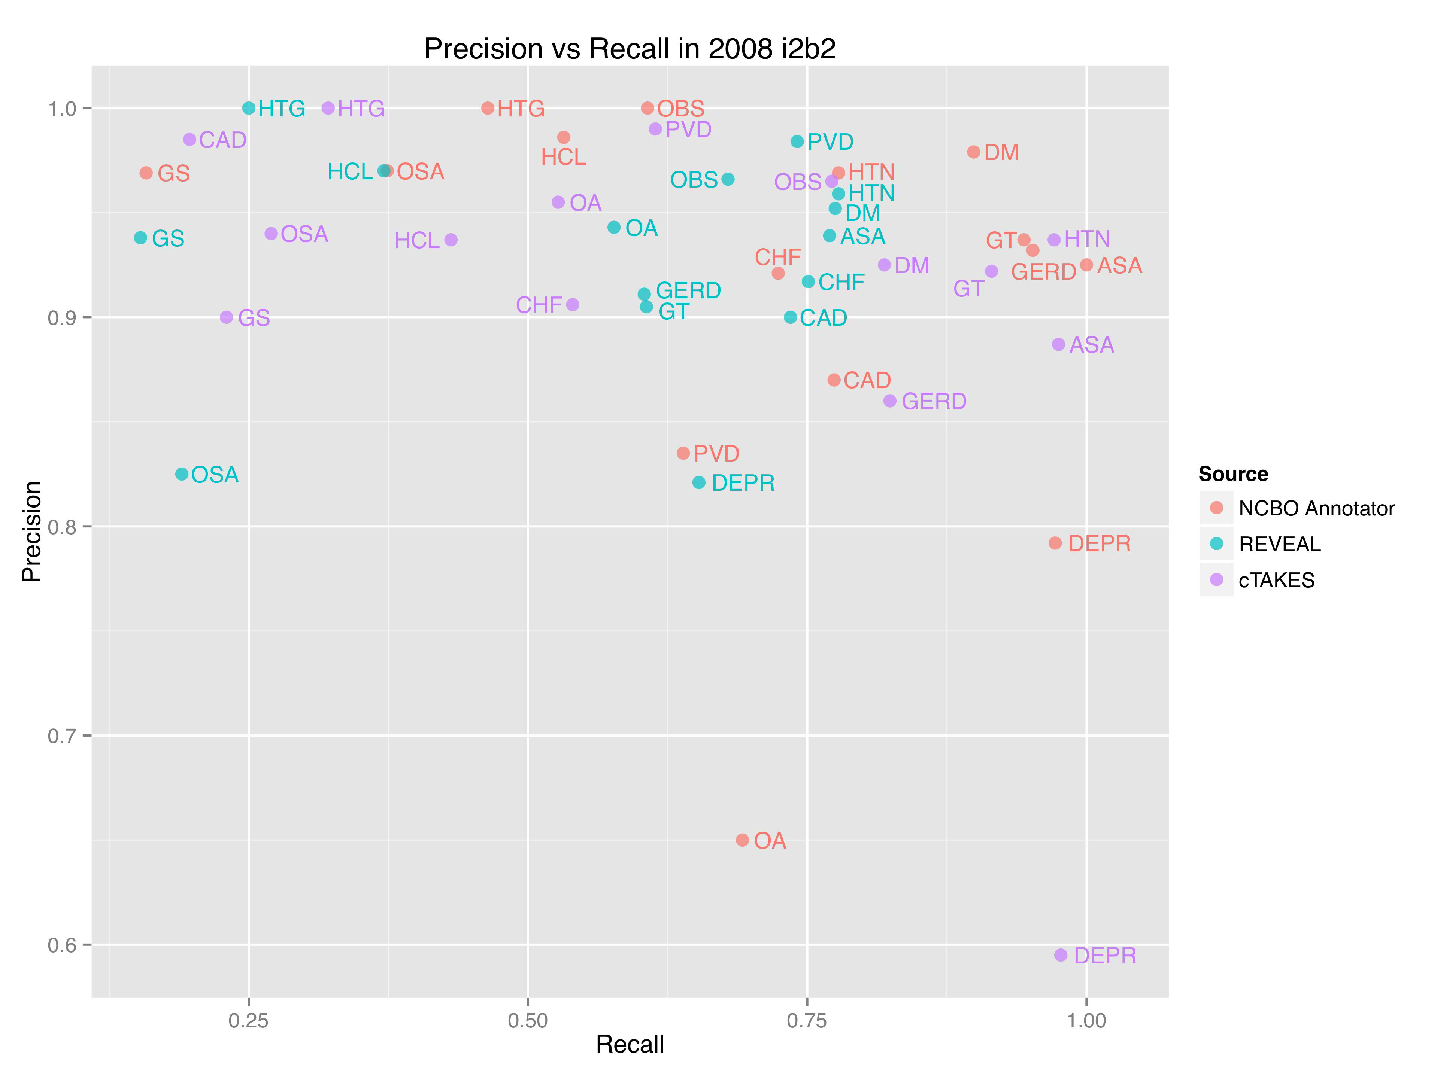
\includegraphics[width=0.9\linewidth]{ch4-figures/Figure2.pdf}
  \end{center}
  \caption[Performance of text processing methods in 2008 i2b2
    Challenge]{The precision and recall of the NCBO Annotator, REVEAL
    and cTAKES in the 2008 i2b2 dataset is plotted here for each
    indication.  There is considerable variation in recall across both
    systems and indications, but generally indications that are hard
    to detect are hard to detect for all systems (e.g., Gallstones –
    labeled here as GS).  There is no universally best system across
    all indications with respect to either precision or recall.
    Labels: ASA=asthma, CAD=coronary artery disease, CHF=congestive
    heart failure, DM=diabetes, DEPR=depression, GS=gallstones,
    GERD=gastro-esophageal reflux disease, GT=gout,
    HCL=hypercholesterolemia, HTN=hypertension,
    HTG=hypertriglyceridemia, OA=osteoarthritis, OBS=obesity,
    OSA=obstructive sleep apnea, PVD=peripheral vascular disease. }
  \label{fig:short}
\end{figure}


\subsection{Safety profiling of Cilostazol}
The goal of this task is to profile adverse events associated with the
use of Cilostazol in patients with Peripheral Arterial Disease.  The
output is odds ratios and confidence intervals for each adverse event.
Figure 4.3 shows results from Leeper et al, which were obtained using
the NCBO Annotator based workflow, along with results from the same
analysis performed using annotations from REVEAL.  There is no
significant difference in either the odds ratios or confidence
intervals for any of the adverse events except for the event ‘sudden
cardiac death’, for which REVEAL found no instances in the data.

\begin{figure}
  \begin{center}
    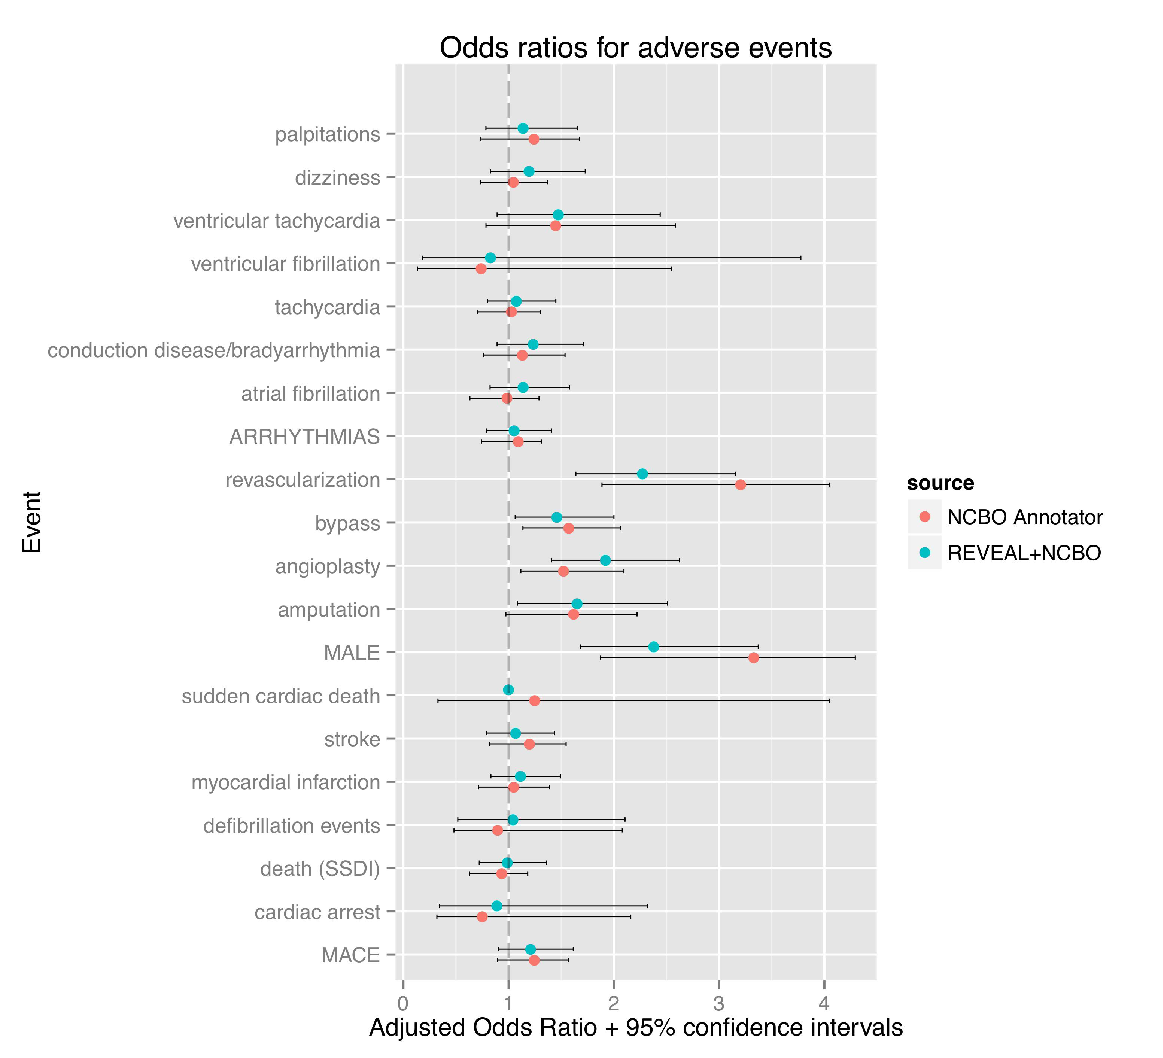
\includegraphics[width=0.9\linewidth]{ch4-figures/Figure3.pdf}
  \end{center}
  \caption[Adverse events in PAD with and without Cilostazol]{Profile
    of adverse events in PAD patients with and without exposure to
    Cilostazol.  The plot shows odds ratios and 95\% confidence
    intervals calculated using annotations from STRIDE using the NCBO
    Annotator based workflow and REVEAL.  There is no change in the
    conclusions of this analysis depending on the text processing
    system being used.  Note that REVEAL did not find any instances of
    “sudden cardiac death” in the data; for this event, we set the
    odds ratio to 1.  }
  \label{fig:short}
\end{figure}


\subsection{Learning adverse drug-drug interactions}
The goal of this task is to use mentions of drugs and indications in
clinical notes from STRIDE to detect adverse drug-drug interactions
following the method of Iyer et al.  The output is a set of adjusted
odds ratios for a gold standard set of known and negative drug-drug
interactions and associated adverse events.  Figure 4.4a shows
Receiver Operator Characteristic (ROC) curves for the gold standard as
we vary the odds ratio threshold for signaling an adverse drug-drug
interaction.  There is no significant difference in the ROC curves
(p-value = 0.275). Figure 4.4b shows the area under the Area Under the
ROC Curve (AUC) for each of 9 adverse events separately.  For all
adverse events, there is no significant difference in the AUC between
the two systems.  Note that this analysis excludes the adverse event,
“serotonin syndrome”, for which the NCBO Annotator is significantly
better than REVEAL (p-value < 1e-6).

\begin{figure}
  \begin{center}
    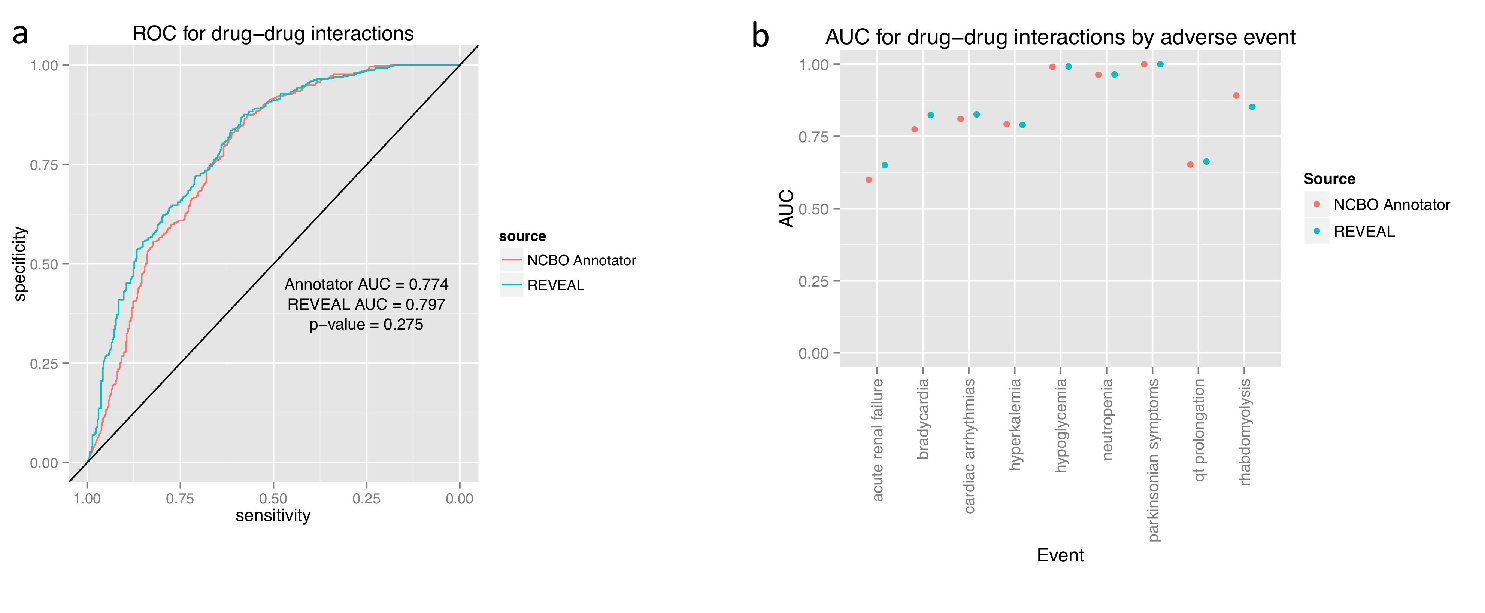
\includegraphics[width=0.9\linewidth]{ch4-figures/Figure4.pdf}
  \end{center}
  \caption[Detection of adverse drug-drug interactions]{Detection of
    adverse drug-drug interactions.  The analysis of Iyer et al was
    carried out using either the NCBO Annotator based workflow or
    REVEAL to process clinical notes from STRIDE.  (a) There is no
    significant difference in the ROC curves (p-value = 0.275 by
    DeLong’s test) for the two systems.  (b) AUCs for each of 9
    adverse events separately.  For all adverse events, there is no
    significant difference in performance (p-values > 0.05).}
  \label{fig:short}
\end{figure}


\subsection{Learning used-to-treat relationships}
The goal of this task is to use mentions of drugs and indications in
clinical notes from STRIDE to construct features that are useful for
identifying which drugs are being used to treat which indications,
according to the methods in Jung et al.  The output is a set of
performance metrics for an SVM classifier, including positive
predictive value, specificity, sensitivity, and F1 based on a hold out
test set. Figure 4.5 shows the performance of classifiers trained and
tested using features derived from the NCBO Annotator based workflow
and REVEAL), and shows that there is no significant difference in
performance (p-value = 0.29 by McNemar’s test).

\begin{figure}
  \begin{center}
    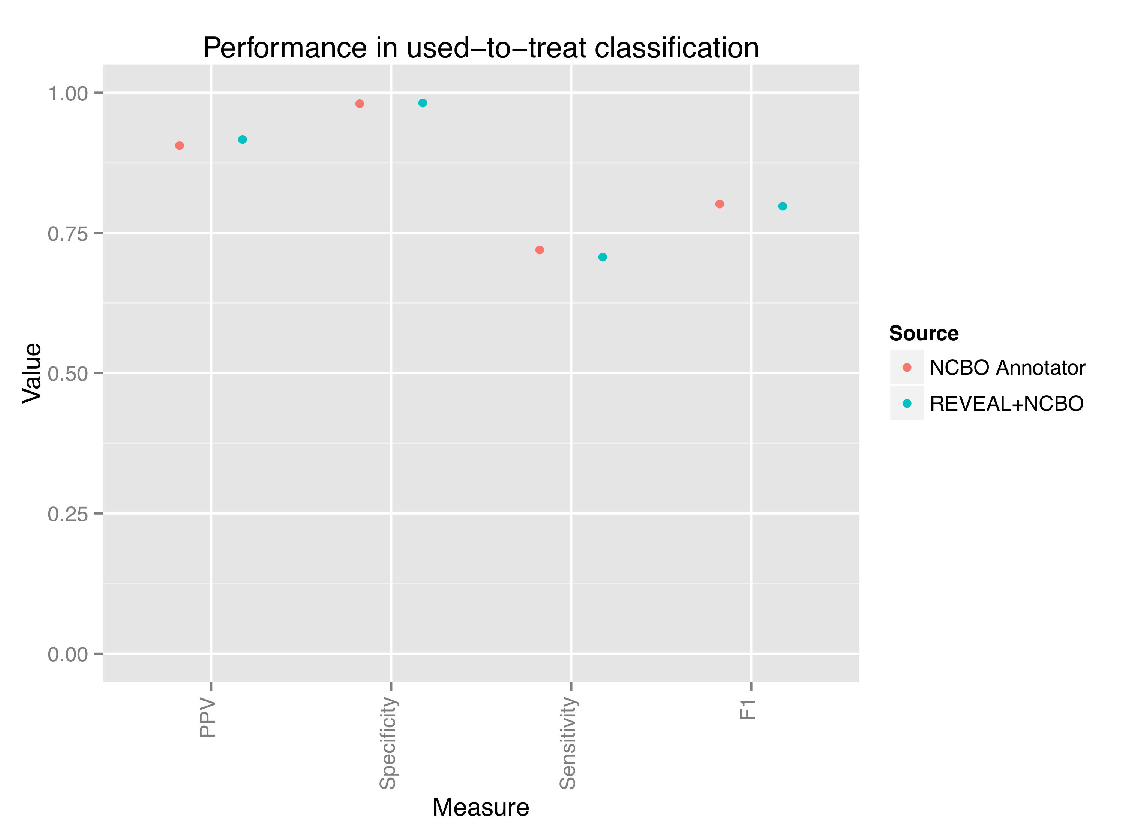
\includegraphics[width=0.9\linewidth]{ch4-figures/Figure5.pdf}
  \end{center}
  \caption[Detecting used-to-treat relationships]{Detecting
    used-to-treat relationships.  We carried out the analysis
    described in Jung et al using either the NCBO Annotator or REVEAL
    to annotate clinical notes from STRIDE.  There is no significant
    difference in performance between classifiers trained and tested
    using features derived from either (p-value = 0.29 by McNemar’s
    Test).}
  \label{fig:short}
\end{figure}


\subsection{Learning used-to-treat relationships with limited data}
We explored whether or not more advanced NLP methods, as embodied in
REVEAL, are advantageous when data is limited so that rare
associations are less well represented in the data.  Figure 4.6 shows
the relationship between dataset size and accuracy of the classifiers
in the used-to-treat task.  Each plot shows the mean performance and
standard error of the mean over ten random samples of patients.  The
gap in accuracy as the dataset size decreases remains quite modest,
even at only 1/64th of the dataset size.  However, the classifiers
trained on output from REVEAL consistently show higher sensitivity
with smaller datasets starting at datasets ¼ the size of the full
dataset.  This ¼ size corresponds to roughly 2.25 million notes, which
would correspond to approximately 250,000 patients if each patient had
the median number of notes. These results agree with the notion that
more advanced NLP will be advantageous when detecting rare
associations or when data is limited.

\begin{figure}
  \begin{center}
    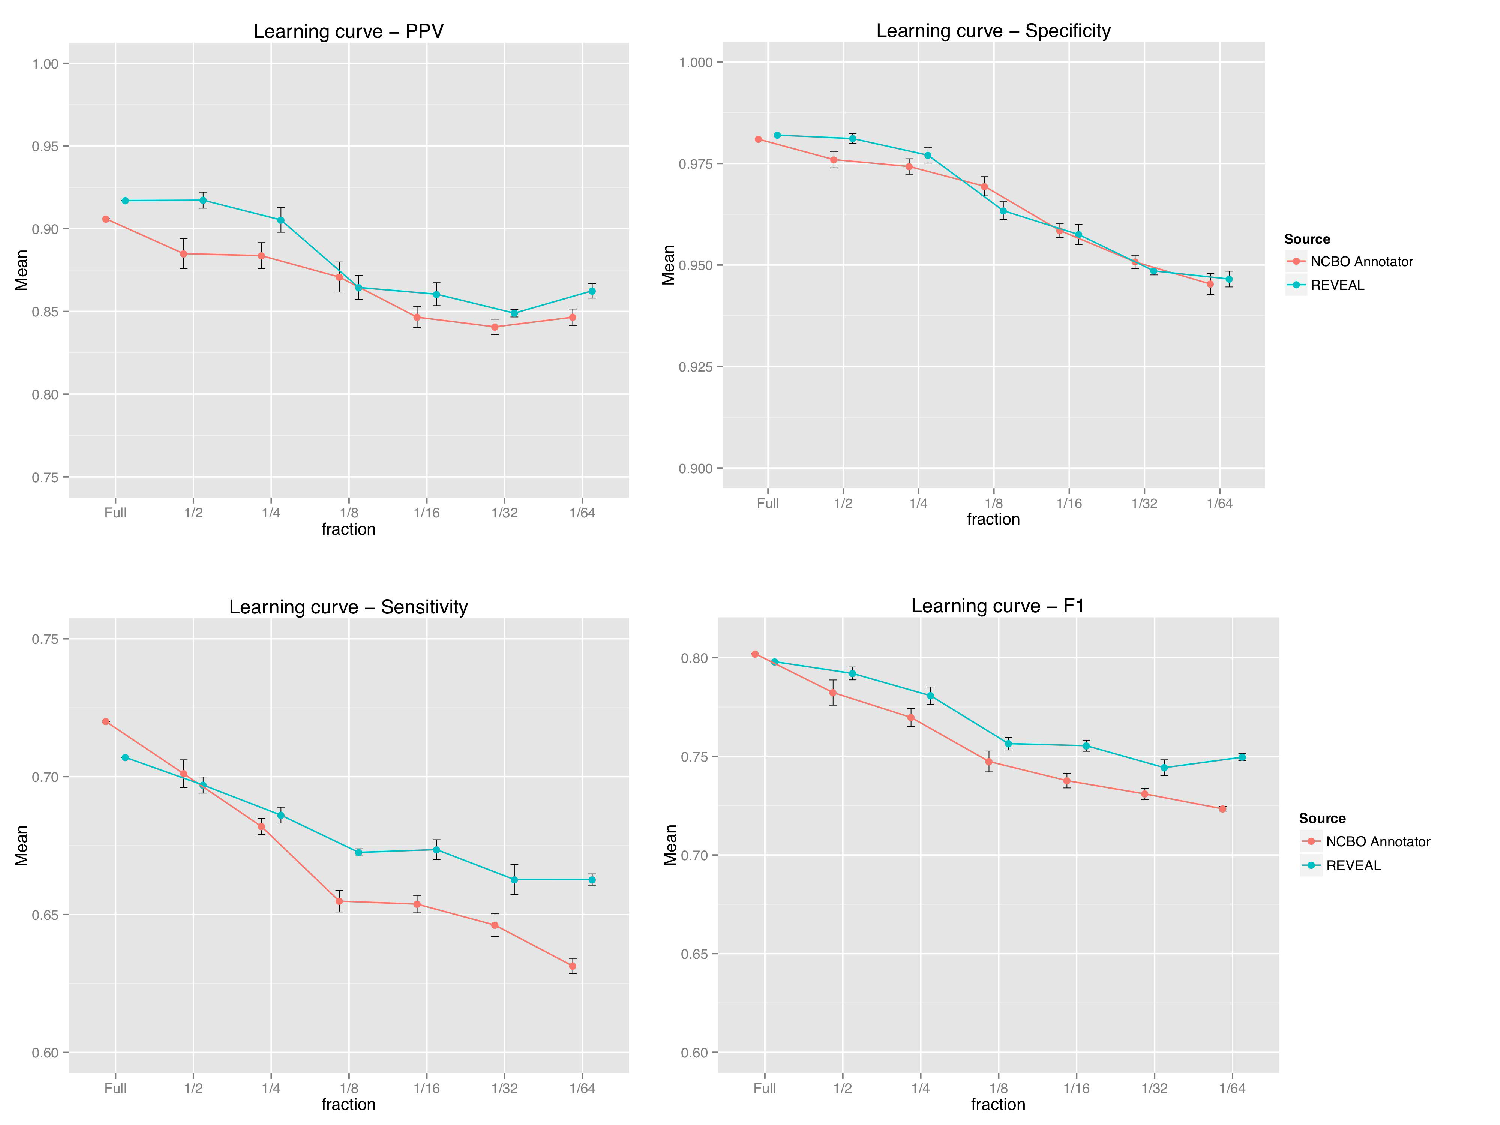
\includegraphics[width=0.9\linewidth]{ch4-figures/Figure6.pdf}
  \end{center}
  \caption[Learning used-to-treat relationships with limited
    data]{Learning curves for the used-to-treat task. We sampled
    random subsets of patients and used the associated notes to
    generate features based on the annotations of those notes by
    either the NCBO Annotator or REVEAL.  This was repeated 10 times
    for each fraction of the full STRIDE dataset.  The mean
    performance metric across the 10 runs is plotted, along with the
    standard error of the mean.  REVEAL has higher sensitivity in
    smaller datasets, and generally has higher precision/PPV.}
  \label{fig:short}
\end{figure}


\section{Discussion}
Recognizing mentions of drugs and diseases in clinical text is a key
step in using the unstructured text from EHRs to address many
questions of clinical interest.  In this paper, we have performed a
systematic comparison of the tradeoff between simple term recognition
and the deeper linguistic understanding of clinical text provided by
advanced NLP, as embodied by the NCBO Annotator and REVEAL
respectively.  The NCBO Annotator uses mgrep and an extensive
dictionary mapping strings to biomedical concepts, along with the
NegEx negation detection module, to efficiently find mentions of the
concepts in text.  In contrast, REVEAL performs extensive
preprocessing, including parsing, word sense disambiguation, and other
core NLP tasks en route to identifying mentions of drugs and diseases.
It is significantly more computationally expensive than the NCBO
Annotator based workflow. For example, the average time to process one
clinical note using REVEAL is 10 seconds, whereas with the NCBO
Annotator based workflow it is 0.01 seconds.  Furthermore, the NCBO
Annotator is a freely available tool while REVEAL is a commercial
product.  These tools were evaluated on a set of clinical research
tasks – safety profiling of Cilostazol, learning adverse drug-drug
interactions, and learning used-to-treat relationships between drugs
and diseases.  We also evaluated the accuracy of the systems in
finding positive mentions of 16 diseases in a manually annotated set
of clinical notes from i2b2.  We found little difference in accuracy
between the methods in any of the three clinical research tasks.

The clinical research tasks we undertook used aggregate statistics
over an entire corpus of clinical text.  In such tasks, all that
matters is that we accurately count mentions of drugs and indications
in the text.  We note that the best performing systems in the textual
portion of the 2008 i2b2 Obesity Challenge were similar in spirit to
the NCBO Annotator \cite{Uzuner2009}.  In the summary paper on that
challenge \cite{Uzuner2011}, Uzuner writes, “Most of the factual and
objective pieces of information were identified by simple rule-based
systems armed with dictionaries of terms and negation extraction
modules”.  Our findings mirror that viewpoint and it seems that for
the set problems we examined, having a good negation detection module,
a comprehensive dictionary, and a best-effort mapping of strings to
concepts are the key ingredients necessary for excellent accuracy.
More advanced NLP techniques do not appear to add much value to such
tasks, and take a much longer time to run.  We note that using REVEAL
to find strings of interest, and then using our mapping of strings to
concepts consistently performed better at the i2b2 annotation task
than the default mapping provided by REVEAL itself.  This suggests
that the quality of the mapping of strings to concepts is one of the
key differences between the systems.  In work evaluating extensions of
cTAKES for document classification, Garla et al found that much of
their tuning consisted of adding terms and lexical variants of terms
to their dictionary \cite{Garla2011}.

These results do not mean that the simple approach embodied by
dictionary based approaches, such as the NCBO Annotator, is
necessarily best for all problems.  For instance, the used-to-treat
task is formulated as a population level problem instead of asking
whether a drug is being used to treat a disease as asserted in a
particular note.  For the latter type of question, in which we want to
infer complex relationships between entities within a given text, the
richer linguistic information output by a full NLP system, such as
part of speech tags, a dependency parse, etc, can be very useful
\cite{Goldstein2009}.  Furthermore, we found that features derived
from REVEAL were more predictive of the used-to-treat relationship
than features derived from the NCBO Annotator based workflow as we
decreased the size of the dataset.  This is consistent with the
intuition that as the dataset size decreases, rare associations may be
more difficult to detect using simple text processing methods.  Thus,
it may be worthwhile to use a full-featured system when the dataset is
relatively small.  It should also be noted that while the upfront
computational cost of running REVEAL on a large corpus may appear
large, it is a one-time cost.  And finally, we note that the systems
were used “out of the box” (i.e., without any special tuning for the
evaluation tasks).  Given that the analysis methods were originally
developed for dictionary-based approaches they could be more effective
in using that output.  It is certainly possible that different methods
that take explicit advantage of the richer information provided by
more advanced NLP methods could outperform the original
methods. However the gain would come at a significant computational
cost, and require expertise that currently only exists in specialized
NLP research teams.

These caveats notwithstanding, our results suggest that for a variety
of questions of clinical interest, it is feasible to use very simple
and fast approaches in lieu of more complex approaches in deriving
useful information from the unstructured data in EHRs.

\section{Conclusion}
Widespread adoption of EHRs is creating a new source of data as a
by-product of routine clinical care.  This data is increasingly
recognized as an asset that can be used to address problems in public
health, health care economics, quality of care, drug safety
surveillance, and even personalized medicine
\cite{Pathak2013,Pathak2013b,Denny2013,Jensen2012,Murdoch2013,Murff2011,Shah2013}.
However, extracting actionable information from EHRs is a challenging
problem because much of its value resides in unstructured text.  NLP
has been applied to this problem to good effect.  In this paper, we
have explored the tradeoff between using a free, simple but fast term
recognition system and a more advanced commercial NLP system.  We
evaluated the systems in a variety of tasks that address questions of
clinical interest.  These tasks ranged from canonical studies that use
the mentions of drugs and diseases to calculate odds ratios, such as
assessing the safety profile of a particular drug in a well-defined
patient population, to a machine learning approach to finding
used-to-treat relationships at the population level.  We achieve the
same accuracy in all three clinical research tasks


\chapter{Prediction of Delayed Wound Healing}
\section{Introduction}
\subsection{Chronic wounds}
Chronic wounds are those that fail to heal in a timely manner
\cite{Lazarus1994}, and affect an estimated 6.5 million people in the
United States (2\% of the population) \cite{Fife2012}.  Chronic wounds
are at increased risk of complications, such as amputation and
infection, which can have a severe negative impact on patient
well-being.  The cost of treating these wounds is high – up to \$50
billion annually \cite{Driver2010,Hess1996,Kuhn1992} – and the
incidence of chronic wounds is expected to increase due to an aging
population and rising risk factors such as diabetes and obesity
\cite{Sen2009}. Given accurate prognostic information, it may be
possible to triage patients for additional care such as additional
monitoring and at-home care, hyperbaric oxygen therapy (HBOT), and
negative pressure wound therapy (NPWT)
\cite{Andros2006,Clemens2008,Melling2006,Stojadinovic2008,Wu2008,Armstrong2008,Bozzuto2000}.
Thus an accurate prediction has the potential to change the course of
clinical treatment.

Previous work has attempted to identify factors of prognostic value in
predicting delayed wound healing, but most of these studies were
restricted to specific wound types such as venous leg ulcers
\cite{Margolis2003,Margolis2004,Cardinal2008,Ubbink2013,Kantor1998,Wicke2009}.
They used patient cohorts of modest size and drawn from single sites
or enrolled in clinical trials, limiting the generalizability of these
results to the diversity of patients and wound types seen in clinical
practice \cite{Carter2009}.  Furthermore, these models have not yet
been validated in independent datasets with respect to either
discriminatory power or calibration.

Among the best work to date is that of Margolis et
al. \cite{Margolis2003,Margolis2004} who developed prognostic models
for venous leg ulcers and diabetic neuropathic foot ulcers using data
from tens of thousands of patients across geographically diverse
outpatient wound care centers, and carefully validated the models,
achieving excellent calibration but only modest discriminative power
(AUCs ranging from 0.63 to 0.71).  These results led to the study by
Kurd et al. \cite{Kurd2009}, a clustered multicenter trial
demonstrating that providing prognostic information from these models
to clinicians improved healing rates even without specific guidance
about treatment options.

In this work, we report the development and validation of a novel
prognostic model that uses data routinely collected over the first
week of care at outpatient wound centers.  Our model achieves an AUC
of \textbf{CHANGE ME} 0.863 (95\% confidence interval 0.857-0.869) on
held out data and provides well-calibrated probabilities for delayed
wound healing.  Our model is constructed and validated on a dataset
comprising tens of thousands of patients with over a hundred thousand
wounds from geographically diverse wound care centers.  All wound
types are considered in this work, and thus the model is applicable to
the full diversity of wounds seen in clinical practice.

\subsection{Impact of Non-stationarity on Predictive Modeling}
The rapid adoption of electronic health records (EHRs) is a key
enabler of the learning healthcare system
\cite{Friedman2010,Weng2012,Shah2012,Bates2014,Embi2013}.  The most
immediate effect of EHR adoption is simply to vastly increase the
amount of data available for tasks such as predictive modeling of
clinical outcomes.  This increase in data enables developers of such
models to employ increasingly sophisticated models to improve
performance while still controlling for overfitting.  For example,
recent work has applied tensor factorization to discover latent
disease subtypes \cite{Ho2014}.  Such models are a far cry from the
logistic regression models that have long been a mainstay of clinical
research, and have the potential to transform clinical care.  However,
the nature of EHR derived data raises several practical issues in the
development of such models \cite{Hersh2013,Hripcsak2011,Paxton2013}.
Failure to take these issues into account in the development and
deployment of these models could lead to high profile failures that
could ultimately delay the learning healthcare system
\cite{Cook2011,Boland2013}.

EHR records typically have repeated observations of a constantly
evolving set of patients.  Furthermore, we note that the health care
system in the United States is currently, and for the foreseeable
future, in a state of flux, with new systems being adopted and
clinical practice evolving at a rapid pace as incentives change.
Indeed, we note that this situation is in fact an explicit goal of the
learning health care system.  We explore what such changes imply for
predictive modeling using EHR data.

The wound healing dataset we use to develop a predictive model
consists of wound and patient data collected over the course of care
at outpatient would care centers operated by Healogics Inc between
2009 and 2013.  In this setting, patients are seen on a weekly basis
to monitor the progress of wound healing and adjust care as
appropriate.  Quantitative and categorical descriptions of wounds are
entered into an EHR during each such assessment.  The objective of the
model is to predict whether or not a given wound will be an outlier
with respect to how long it takes to fully heal, given only
information collected during the first and second wound assessments.
The threshold for delayed wound healing was set to fifteen weeks based
on the observations of clinical experts at Healogics.

This dataset has several characteristics that we believe make it
especially illuminating with respect to developing and potentially
deploying predictive models in practice.  First, the dataset consists
of longitudinal observations of multiple wounds from many patients,
with no restrictions on the patient population or wound types.
Second, the data was collected from 68 geographically distributed
wound care centers.  Finally, Healogics expanded its operations by
both opening new wound care centers and taking over the operations of
other specialized wound care systems during the study period.
Healogics was also increasing adoption of its EHR, and it was apparent
from preliminary examination of the data that there were significant
changes in EHR use over the study period.  For instance, prior to 2013
there were many instances of wounds whose type was coded as ‘Diabetic
Wound, Lower Extremity’.  From 2013 onwards, this wound type almost
entirely disappeared, and was superseded by more specific categories
such as ‘Neuropathic diabetic wound’ and ‘Neuro-ischemic diabetic
wound’.  More generally, the prevalence of delayed wound healing was
lower in 2013 (i.e., the most recent data available for this study)
than previously (10.4\% versus 13.2\% respectively).  Thus, in this
dataset, there was significant non-stationarity, i.e., the process
generating the data changed over time.  This issue has long been known
to bedevil predictive models in other domains but receives relatively
little attention in the biomedical informatics literature
\cite{Bickel2009,Hoens2012,Moreno2011}.

We present experiments evaluating the impact of non-stationarity on
discriminative power (how well models distinguish between cases and
non-cases) and on model calibration (how closely the posterior
probabilities of delayed wound healing output by models match observed
frequencies of delayed wound healing).  We approximate different
degrees of stability of the data generating process by changing the
way that the data is split into training and test sets. We then
examine how such change impacts model selection.  To that end, we
consider the use of increasingly sophisticated models, starting from
regularized logistic regression, progressing through non-linear models
capable of automatically modeling interactions between predictors, and
ending with ensemble methods that combine the predictions of many base
models.  Finally, we examine the impact of non-stationarity on
engineered, domain specific features.

We demonstrate that in a setting that approximates a stationary data
distribution, ensemble methods such as stacking can provide
significant boosts to predictive power.  However, this performance
gain disappears when the data distribution is non-stationary.  In both
cases, however, there is consistent benefit from using engineered,
domain specific features.  We find that using non-linear models that
capture feature interactions automatically is useful in this dataset
but that the benefit from such models is reduced under
non-stationarity.  Our findings emphasize the importance of matching
the model development process with the intended use of the model. If
the model is intended for use on future patients, it is critical to
take non-stationarity into account to obtain a reliable estimate of
model performance.

\section{Materials and Methods}
Our goals are two-fold.  First, we aim to develop an accurate,
well-calibrated model for predicting delayed wound healing.  We also
aim to investigate the impact of non-stationarity on such models.  The
outcome we are trying to predict is whether or not a given wound will
take longer than 15 weeks to heal using information routinely
collected during the first week of care. We approach this by fitting a
series of increasingly complex models—with and without domain specific
features—to different training and test splits of the data.  We
observed that the dataset exhibits substantial non-stationarity.  We
can, however, control the degree of non-stationarity seen by the
models by changing the way we split the data.  We evaluate the models
for discriminative power and calibration under these different
conditions.  In the remainder of this section, we provide details
about the dataset, feature construction, model development and
evaluation.

\subsection{Dataset}
The dataset is comprised of 1,182,751 time-stamped wound assessments
performed at 68 Healogics outpatient wound care centers distributed
over 26 states from 2009 through 2013 (Figure 5.1).  These wound
assessments represented 180,716 unique wounds.  Each wound assessment
consists of both quantitative information regarding a specific wound,
such as length, width, depth and area, in addition to categorical
descriptors such as wound type, anatomical location, presence/absence
of erythema and ICD9 codes associated with the assessment.  Each
assessment is also associated with unique wound and patient keys,
allowing us to associate each wound with basic demographic information
such as age, gender, and insurance status along with its
outcome. Wound assessments were performed approximately weekly, and
the dataset spans 2009 through 2013.  There were 40 wound types (e.g.,
Pressure Ulcer, Venous Ulcer) and 37 anatomic locations.  The mean
duration of care was 52.2 days.  Overall, 11.6\% of wounds exhibited
delayed wound healing, defined as 15 or more weeks to closure. A total
of 59,958 patients are represented.  Figure 5.2 shows basic statistics
about the dataset.

\begin{figure}
  \begin{center}
    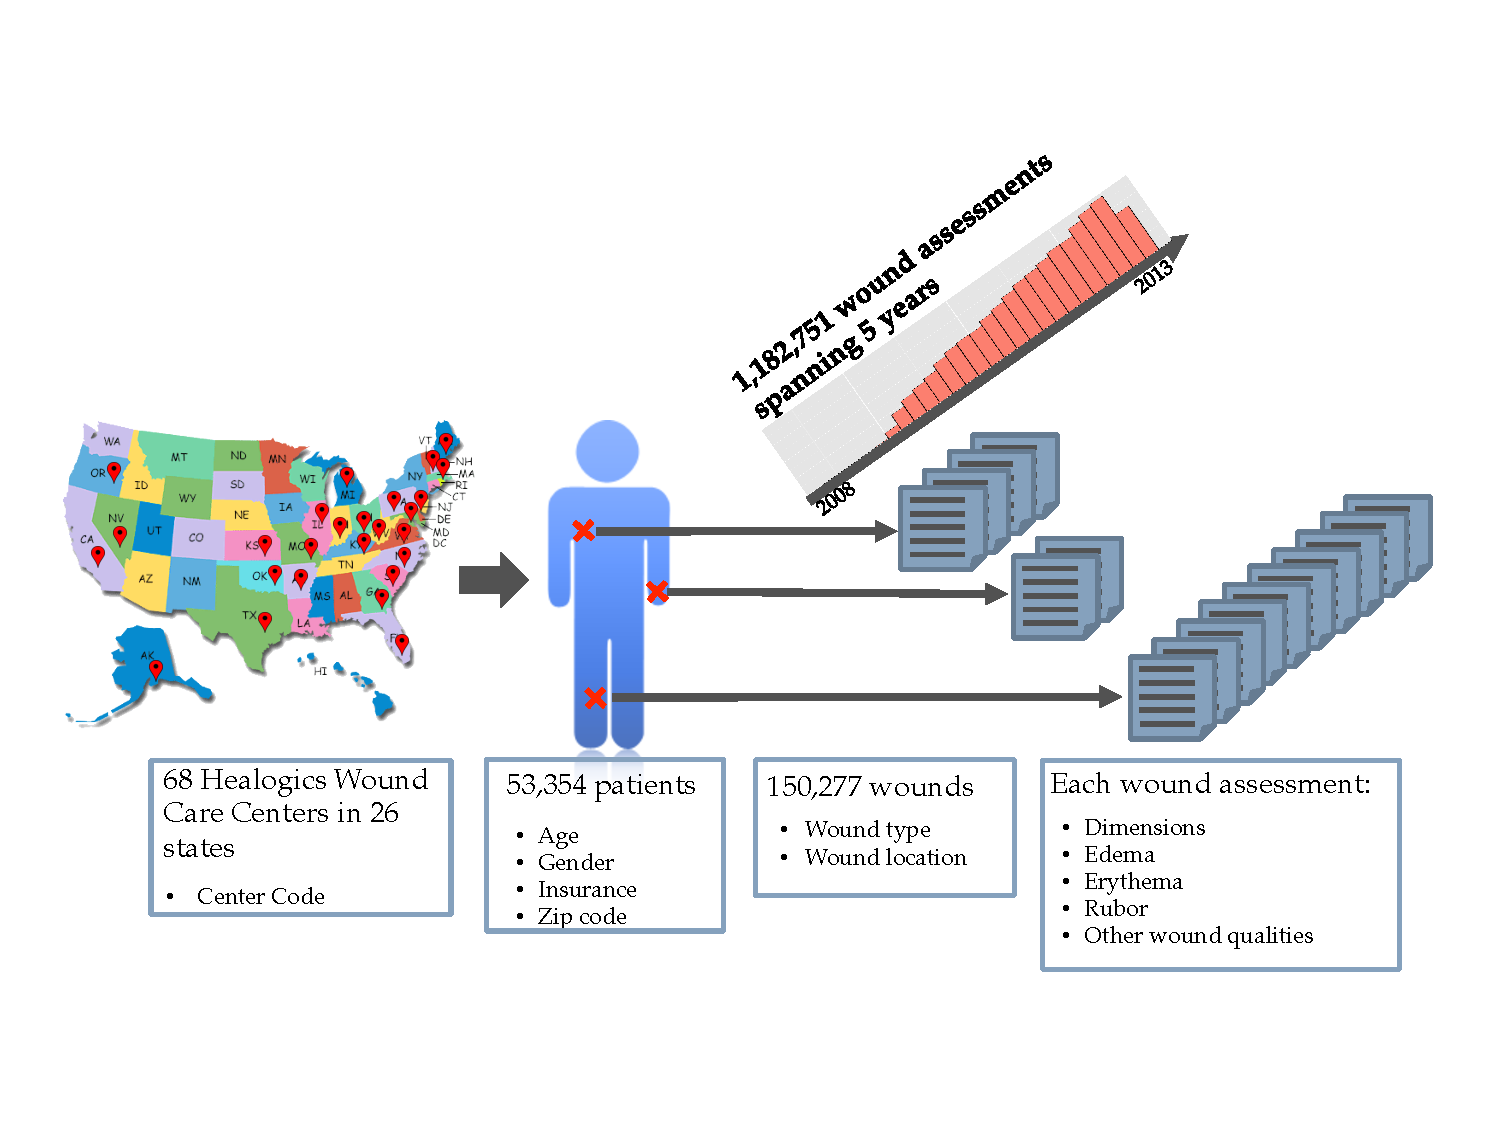
\includegraphics[width=0.9\linewidth]{ch5-figures/dataset_overview.pdf}
  \end{center}
  \caption[Wound healing dataset characteristics]{Dataset
    characteristics. The dataset is drawn from 68 Healogics wound care
    centers in 26 states over a period spanning 2009 through 2013 and
    comprises 181,716 wounds from 59,958 patients. Patient and wound
    information is recorded in an EHR at each weekly wound
    assessment. There were 40 distinct wound types spanning 37
    anatomical locations. We use the information recorded in the first
    two assessments to predict delayed wound healing.}
  \label{fig:short}
\end{figure}

\begin{figure}
  \begin{center}
    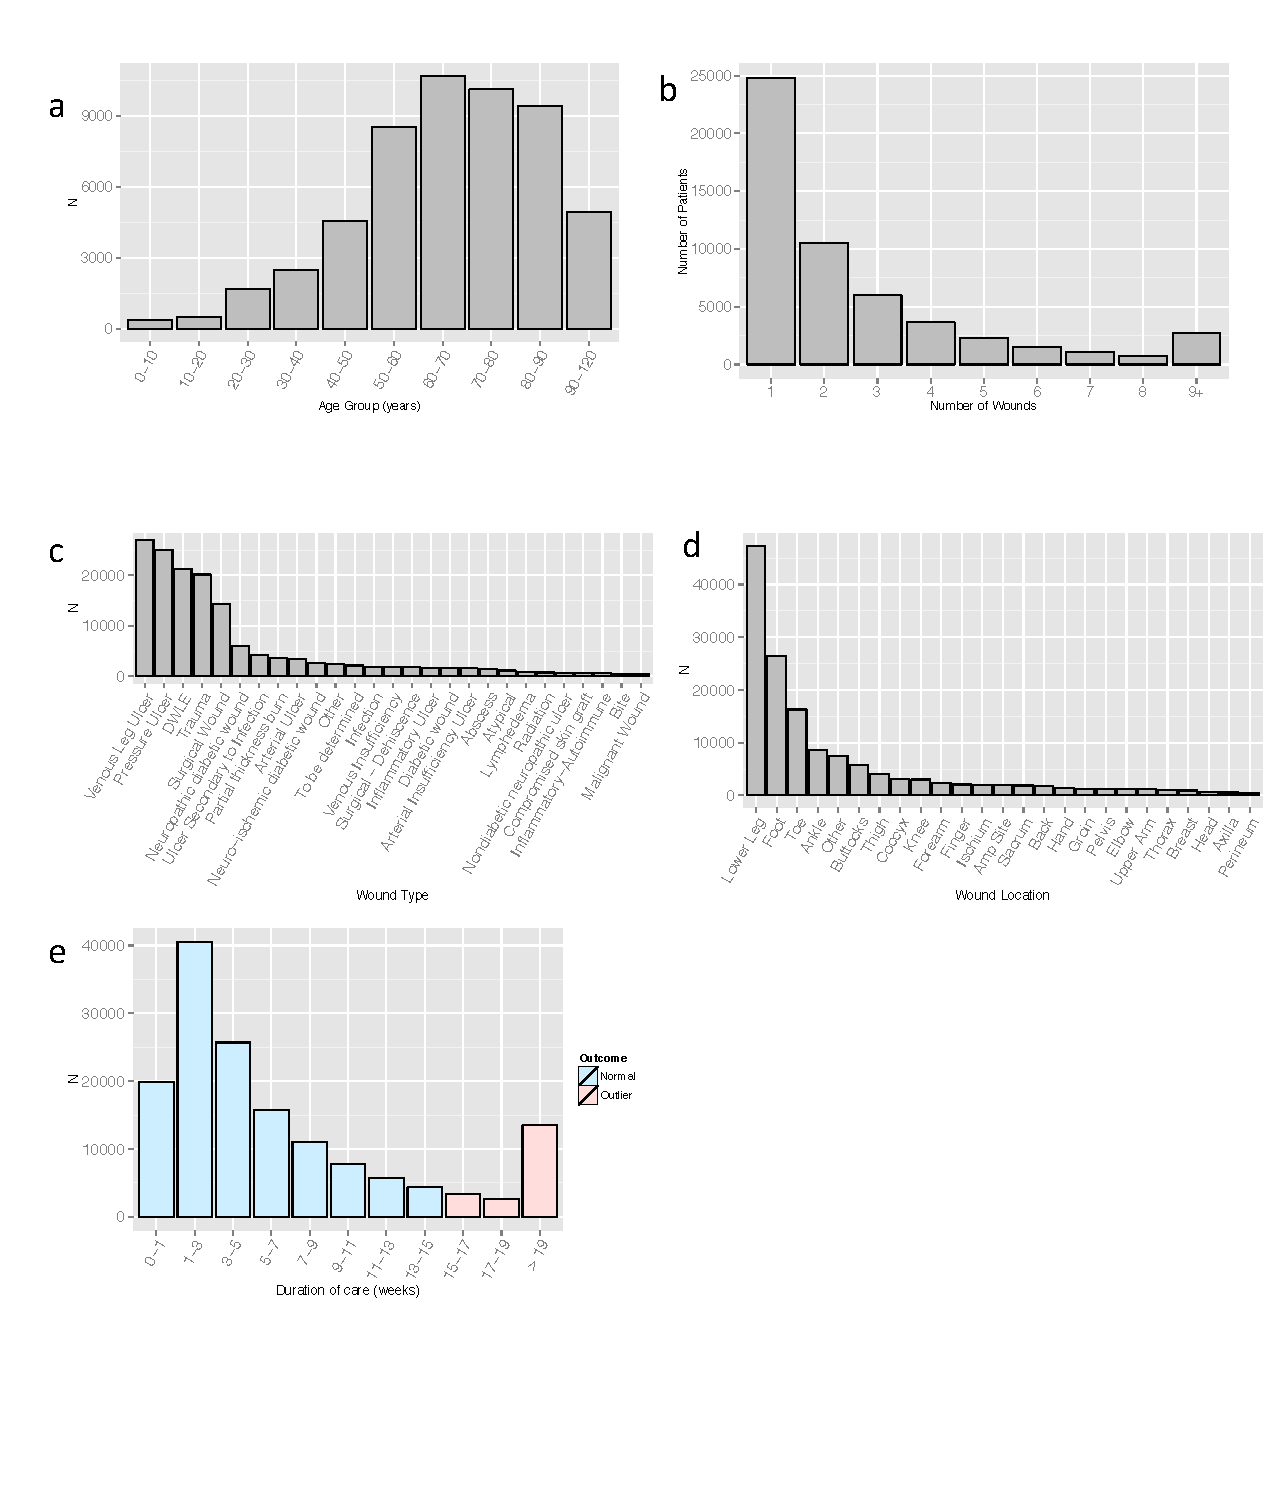
\includegraphics[width=0.9\linewidth]{ch5-figures/dataset_stats.pdf}
  \end{center}
  \caption[Wound healing dataset statistics]{Dataset statistics.}
  \label{fig:short}
\end{figure}

We removed any wounds that were unresolved by the end of the study
period unless the wound was already past the 15-week threshold for
delayed healing.  We also removed wounds with negative or very large
values for quantitative features (> 99.9th percentile) or with clearly
erroneous demographic information such as negative age.  This left us
with 150, 277 unique wounds for use in training and testing our
models.  The basic features for our models are the data for each wound
that is available at the time of the first wound assessment.

We performed additional pre-processing of the dataset as follows.
First, ICD9 codes were aggregated to 3 digit codes.  Second, wound
types and locations were aggregated into 40 and 37 values,
respectively, in order to account for variation between wound care
centers and misspellings.  Third, insurance information was aggregated
into four values - uninsured, private, Medicaid, and Medicare.

In this study, delayed wound healing is defined as taking 15 or more
weeks to heal; this threshold was chosen based on the advice of domain
experts from Healogics.  11.7\% of wounds meet this criterion in the
final dataset.

\subsection{Training and test splits}
We control the degree of non-stationarity seen by the models by
changing the way the dataset is split into training and test sets. A
naive strategy is to randomly assign wounds into the training and test
sets independently of each other, ignoring both time and the fact that
a single patient may have many wounds in the dataset.  This strategy
mirrors the assumption that the training and test data are from the
same distribution, and may be appropriate in settings in which this is
known or strongly suspected to be true.  A second strategy is to split
patients into training and test sets, and then assign wounds to
training and tests sets according to this patient assignment.  This
strategy respects the grouping of wounds by patient, but ignores time.
It approximates the population of patients undergoing a large change
in the future.  It may also yield a pessimistic estimate of model
performance because it is estimated on completely new patients; in
practice, a wound healing prediction model would see a mix of new and
previously seen patients.  Finally, we simulate a prospective setting
by assigning wounds from the end of the study period to the test set.
This procedure ignores the grouping of wounds by patient, but respects
the fact that we wish to make predictions about the future, and not
past events whose outcomes are unknown.  Under this setting, the model
development process “sees” the non-stationarity in the data.  In all
cases, data was split 4:1 into training and test sets.  In the case of
the simulated prospective setting, we performed this split by ordering
the wound assessments in time, and selecting the most recent fifth of
the data for the test set.  Figure 5.3 illustrates the split
strategies.

\begin{figure}
  \begin{center}
    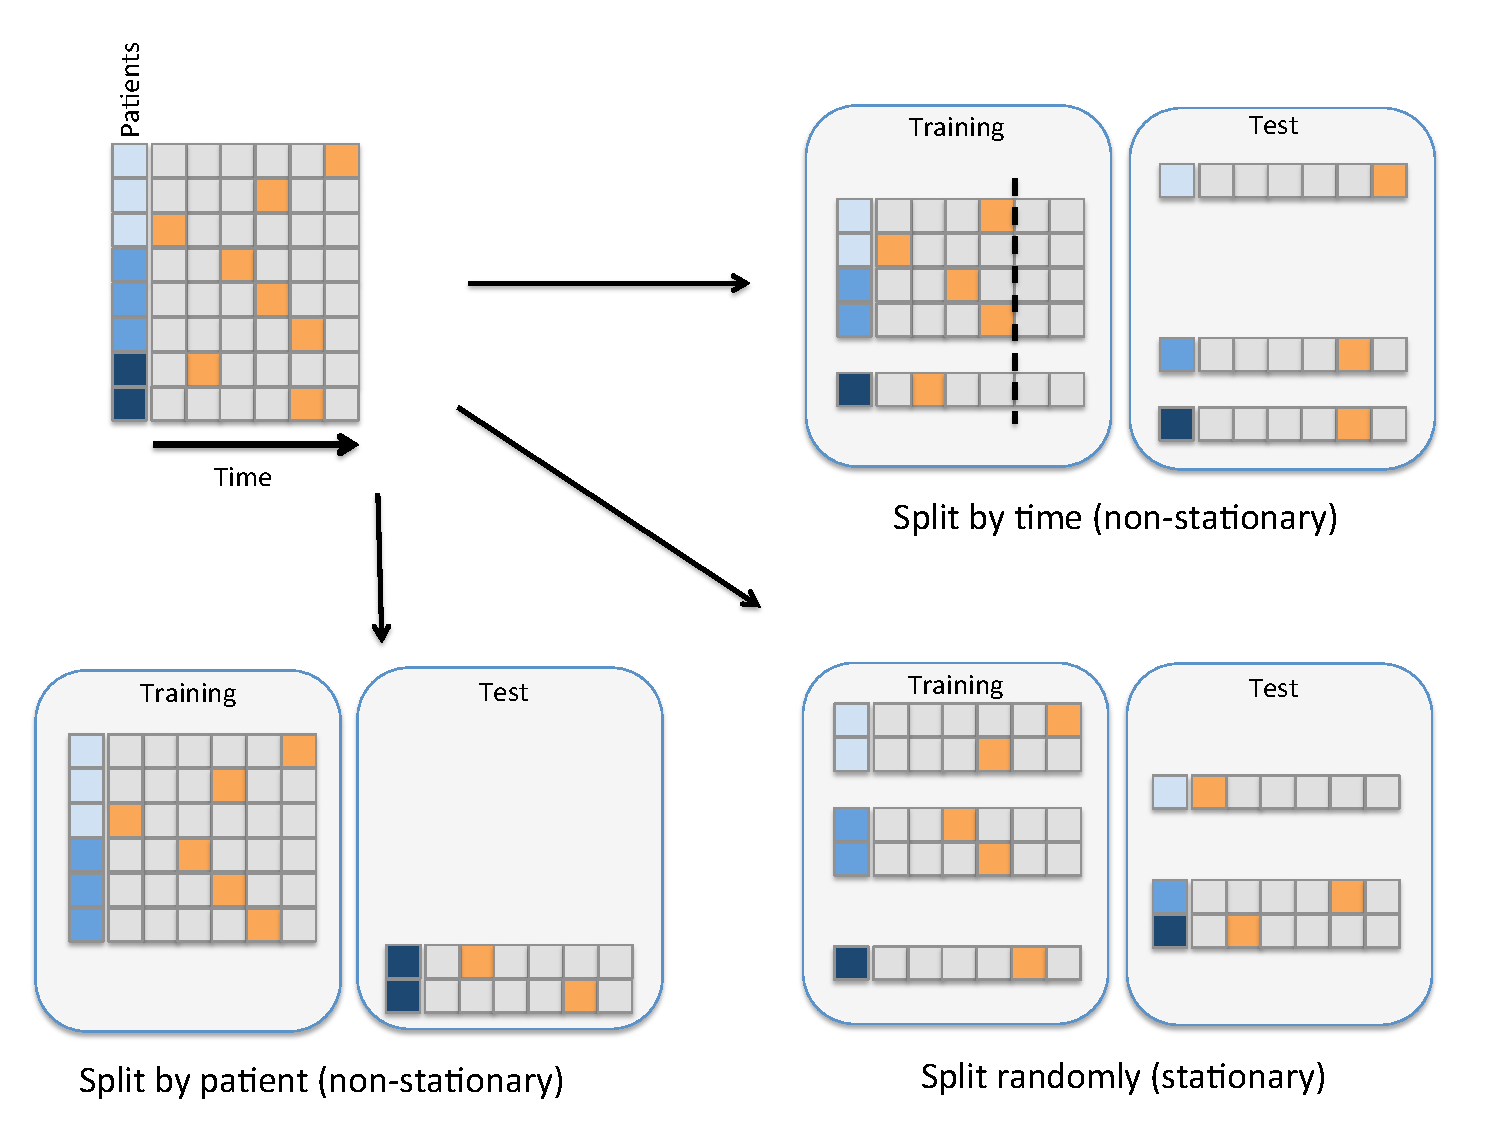
\includegraphics[width=0.9\linewidth]{ch5-figures/train_test_splits.pdf}
  \end{center}
  \caption[Approximating different degrees of stationarity using
    training and test splits] {Approximating different degrees of
    stationarity using training and test splits. Each row represents a
    wound.  The first column represents the patient for a given wound,
    and is color-coded such that different shades indicate different
    patients.  The time of the first wound assessment is indicated by
    the orange cell in the grey columns. In the random split, wounds
    are randomized into training and test directly. In the patient
    split, patients are randomized and wounds from a given patient go
    together. In the prospective split, we assign wounds from the end
    of the study period (shown by the dashed line) to the test set.}
  \label{fig:short}
\end{figure}


\subsection{Model choice}	
We evaluated the following models: L1 regularized linear regression
(LASSO) \cite{Lasso}, random forest (RF) \cite{Breiman2001,Liaw2002},
neural networks (NN) \cite{Goodfellow2013,Pylearn}, and gradient
boosted trees (GBM) \cite{Friedman2001,Ridgeway2007}. Each of these
models were fit to the training set for each of the splits, with their
respective hyperparameters tuned by cross validation on the training
data (LASSO) or on a held out subset of the training data.  Following
hyperparameter tuning, the models were refit to the entire training
set.

We also evaluated the use of two model ensemble methods – model
averaging and stacking – that combine the outputs of the above base
models \cite{Wolpert1992,Ting1999}.  Model averaging simply averages
the predictions of the base models.  We averaged the predictions of
the four base models trained on the full training sets.  In our
stacking experiments, we further split the training sets into two
parts – one for training base models, and another for training the
stacked model.  The stacked model was developed by fitting a GBM model
to the stacking dataset, which consisted of the original set of
features plus the posterior probabilities of the base models on the
stacking data.  

\subsection{Feature engineering}
We constructed additional features for each wound that measure the
change in quantitative variables such as wound dimensions between the
first and second assessments, and features that summarize the total
wound burden of each patient at the time of the first assessment, such
as number of wounds and total surface area. These features capture
intuition such as wounds that are decreasing in size during the first
week are more likely to heal well.  In all, a total of 833 features
were calculated for each wound, the bulk of which were binary
indicators for the levels of categorical variables (31 quantitative
versus 802 binary).

\subsection{Model evaluation}
A useful prognostic model for delayed wound healing should meet two
criteria.  First, it should be able to discriminate between positive
versus negative cases of the delayed wound healing.  Second, it should
output well-calibrated posterior probabilities of delayed wound
healing, i.e., the observed frequency of delayed wound healing should
be close to the predicted probability.  We evaluated the test set
performance of the various models under each all combinations of
training-test splits and feature sets.  Discriminative power on the
test data was evaluated using the Area under the ROC Curve (AUC),
which summarizes the sensitivity-specificity trade off across the
range of possible thresholds for calling an example a positive case.
We obtained 95\% confidence intervals for the AUCs by bootstrapping on
the test set.

Model calibration was evaluated by Brier reliability on the test data.
Brier reliability is a measure of calibration for probabilistic
predictions that are stratified into discrete groups, with lower
values indicating better agreement between the predictions in each
stratum and the observed frequency in those strata
\cite{Stephenson2008}.  It is equivalent to the mean squared deviation
between the predicted probability and the observed frequency within
each stratum, weighted by the number of observations in each stratum.
We formed strata by dividing the interval [0,1] into ten equal sized
bins.  In other words, all samples with predicted probabilities
between 0 and 0.1 fall into one bin, between 0.1 and 0.2 in the next,
etc.  We also evaluate calibration visually, by plotting reliability
diagrams: for each bin, the mean predicted probability is plotted
against the observed fraction of delayed wound healing
\cite{Degroot1982}.  Well-calibrated models will thus have its
reliability diagram near the diagonal line.

\section{Results}

\subsection{Discrimination}
Our measure of discriminative power is AUC in the test set (Figure
5.3), with 95\% confidence intervals obtained by bootstrapping for
10,000 iterations.  If the data generating process is stationary,
i.e., we split the dataset into training and test sets without using
patient and temporal information, we find that the non-linear models –
random forest, neural networks, and gradient boosted trees – have a
significant edge over the linear model (AUCs of 0.861, 0.854, and
0.861 versus 0.827 respectively).  Furthermore, combining the outputs
of these base models by model averaging and stacking provide
additional benefit over these non-linear models (AUCs of 0.872 and
0.876 respectively). These results suggest that one should use the
most complex model, the stacked GBM.

\begin{figure}
  \begin{center}
    \includegraphics[width=0.9\linewidth]{ch5-figures/discrimination.pdf}
  \end{center}
  \caption[AUC of models under different train-test splits]{AUC of
    models under different train-test splits. 95\% confidence
    intervals are shown.  The confidence intervals were obtained by
    bootstrapping on the test set.  }
  \label{fig:short}
\end{figure}

However, under the most realistic training/test split, i.e., a split
in which we trained on older data and evaluated on the most recent
data, we see that the relative performance of the models is almost the
same, with much less difference in performance between the base
models, and no benefit from model averaging and stacking (AUCs ranging
from 0.868 to 0.880 for the base models, and 0.881 for stacking).  We
note that the absolute performance is somewhat higher in the
prospective split setting, but do not generalize from this except to
note that it underscores the importance of non-stationarity.

When training and test data is split by patient, we find that gradient
boosted trees remain the best performing base model but with a smaller
advantage over the other models (AUC of 0.843 for gradient boosted
trees versus 0.819-0.826 for the other base models).  Model averaging
and stacking provide no additional benefit over gradient boosted trees
(AUC 0.846 for stacking versus 0.843 for gradient boosted trees).

We are also interested in the interaction between stationarity and the
use of domain specific features such as those that encode the initial
rate of wound closure.  Without using these features, we observe the
same trends described above, with gradient boosted trees being the
best performing base model under all training/test split procedures,
but with a smaller edge over the other models.  Table 5.1 summarizes
the discrimination performance.

\begin{table}
\begin{center}
  \begin{tabular}{|l|l|l|l|l|l|l||}
    \hline Model & \multicolumn{2}{|c|}{Random split} &
    \multicolumn{2}{|c|}{Prospective split} &
    \multicolumn{2}{|c|}{Patient split} \\
    \hline \hline
    & With & No & With & No & With & No \\
    & engineered & engineered & engineered & engineered & engineered & engineered \\
    & features & features & features & features & features & features \\
    \hline \hline
    Lasso &  0.827 & 0.807 & 0.868 & 0.851 & 0.819 & 0.791 \\
    RF & 0.861 & 0.837 & 0.870 & 0.843 & 0.825 & 0.788 \\
    NN & 0.854 & 0.835 & 0.87 & 0.846 & 0.826 & 0.807 \\
    GBM & 0.861 & 0.834 & 0.880 & 0.859 & 0.843 & 0.807 \\
    Mean & 0.872 & 0.850 & 0.881 & 0.858 & 0.840 & 0.809 \\
    Stacked & 0.876 & 0.875 & 0.881 & 0.860 & 0.841 & 0.808 \\
    \hline
\end{tabular}
\end{center}
\caption{Model discrimination measured by AUC.}
\end{table}

\subsection{Calibration}
Well-calibrated posterior probabilities are desirable for prognostic
models because they enable clinicians and patients to make decisions
that are informed by accurate estimates of the probabilities of the
outcomes of interest, which is especially important when performing
cost-benefit analysis of treatment options
\cite{Cook2007,Cook2008}. We evaluated model calibration by
calculating Brier reliability in the test set (Table 5.2). Here, the
general trend is that under all conditions, the linear and stacked
models are the best calibrated.  Figure 5.5 shows reliability diagrams
for the models under the various conditions.  In Figure 5.5a, we see
that under conditions of stationarity, we observe that the lasso,
neural net, and stacked models all have very good calibration, with
the mean posterior probability of delayed wound healing matching the
observed frequency of delayed healing in each of the bins.  The RF and
GBM models, on the other hand, seem to have relatively poor
calibration.  However, the situation changes under patient and
prospective splits.  Under conditions of non-stationarity, the GBM and
stacked models offer the best calibration.

\begin{figure}
  \begin{center}
    \includegraphics[width=0.9\linewidth]{ch5-figures/calibration.pdf}
  \end{center}
  \caption{Calibration of models under different train-test splits.}
  \label{fig:short}
\end{figure}


\begin{table}
\begin{center}
  \begin{tabular}{|l|l|l|l|l|l|l||}
    \hline Model & \multicolumn{2}{|c|}{Random split} &
    \multicolumn{2}{|c|}{Prospective split} &
    \multicolumn{2}{|c|}{Patient split} \\
    \hline \hline
    & With & No & With & No & With & No \\
    & engineered & engineered & engineered &
    engineered & engineered & engineered \\
    & features & features & features & features & features & features \\
    \hline \hline
    Lasso & 0.000299 & 0.000256 & 0.00146 & 0.00181 & 0.000372 & 0.000339 \\
    RF & 0.00205 & 0.0011 & 0.00347 & 0.00179 & 0.00163 & 0.00152 \\
    NN & 0.000151 & 0.000136 & 0.0021 & 0.000888 & 0.000194 & 0.000732 \\
    GBM & 0.00199 & 0.00227 & 0.000549 & 0.000702 & 0.000127 & 0.0000537 \\
    Mean & 0.00175 & 0.00161 & 0.00215 & 0.00147 & 0.000764 & 0.000602 \\
    Stacked & 0.0000793 & 0.000075 & 0.000401 & 0.000877 & 0.00035 & 0.000234 \\
    \hline
\end{tabular}
\end{center}
\caption[Model calibration measured by Brier calibration]{Model
  calibration measured by Brier calibration.}
\end{table}

\subsection{Model performance}
The goal of developing the model is to be able to predict delayed
wound healing on new wounds in the future.  Therefore, we view the
prospective split as providing the most relevant estimate of model
performance on unseen data.  We now focus on the performance of the
best performing model under the prospective split, gradient boosted
trees (GBM).  The GBM model achieved an AUC of 0.880 (95\% confidence
interval 0.872-0.885) over all wound types.  For the two wound types
previously examined by Margolis et al \cite{Margolis2003,Margolis2004}
(venous leg ulcers and diabetic neuropathic ulcers), we achieve AUCs
of 0.867 and 0.860 respectively, a significant improvement over the
previously reported best results of 0.71 and 0.70.  Performance in
other wound types well represented in the test set (N > 500) ranged
from 0.834 for trauma to 0.878 for pressure ulcers.  Table 5.3 shows
the AUC of this model on the test set by wound type for the ten wound
types most frequent in the test set.

\begin{table}
\begin{center}
\begin{tabular}{|c|c|c|c||}
\hline
&  & \multicolumn{2}{|c|}{AUC} \\
\hline
Wound Type & N & With & No \\
& & delta & delta \\
& & features & features \\
\hline \hline
Venous Leg Ulcer & 3646	& 0.867 & 0.853 \\
Pressure Ulcer & 2991 & 0.878 & 0.850 \\
Trauma & 2715& 0.864 & 0.834 \\
Neuropathic diabetic wound & 2596 & 0.860 & 0.833 \\
Surgical Wound & 1791 & 0.862  & 0.850 \\
Neuro-ischemic diabetic wound & 1180 & 0.874 & 0.838\\
Diabetic wound, lower extremity & 988 & 0.846 & 0.815\\
Abscess & 659 & 0.843 & 0.790 \\
Arterial Insufficiency Ulcer & 593& 0.856 & 0.843 \\
Infection & 381 & 0.826 & 0.806 \\
\hline
\end{tabular}
\end{center}
\caption[Performance of GBM by wound type, prospective
  split]{Performance of the GBM model by wound type under the
  prospective train-test split.  We show results for the ten most
  prevalent wound types in the test set.}
\end{table}

\section{Discussion}
\subsection{A predictive model of delayed wound healing}
We developed a prognostic model for delayed wound healing outcomes
that uses data routinely captured in EHRs during the first two weeks
of care at wound centers.  The model achieves best-to-date
discriminative power and calibration on validation data.  Unlike
previous work, our model is also applicable to the full range of wound
types.  Furthermore, by changing the cutoff threshold, it is possible
to make trade offs between positive predictive value and sensitivity
(recall) for specific uses of the model (Figure 3b).  For instance, it
may be desirable to trade off low positive predictive value for a high
sensitivity when making decisions regarding referral to specialized
wound care centers.  Once referred to a wound center, however, it may
be desirable to have a high positive predictive value and sacrifice
sensitivity when making decisions about high cost interventions that
may improve outcomes in potentially problematic cases.  Because the
model outputs are well-calibrated probabilities, they can be used
directly to make informed referral or intervention decisions that
helps care providers and patients.

Our approach does have limitations. Although our model was developed
on data from 68 geographically distributed wound care centers in 26
states, it may not generalize to centers other than those that
participated in this study.  Indeed, we observe considerable
inter-center variability in practices and patient populations.
Second, it is possible that the model may not generalize to cases
outside wound care centers, limiting its utility for making referral
decisions.  Third, in contrast with previous work, we have traded
simplicity for accuracy.  The simple models by Margolis et al. can be
applied by basic arithmetic.  In exchange, however, we have achieved
significantly higher accuracy.  We would argue that in the age of
widespread and growing adoption of EHRs, it is time to shift some of
the burden of such prognostication to automated systems.

These limitations notwithstanding, our model, to the best of our
knowledge, is the first that has been developed and validated on the
full diversity of patients and wound types seen in clinical practice.
It achieves significantly better discrimination than those of previous
efforts, and is a case study for the meaningful secondary use of
routinely collected EHR data to improve treatment strategies.

\subsection{Non-stationarity in predictive modeling}
The increasing abundance of EHR derived clinical data enables
researchers to apply increasingly sophisticated models to clinical
problems.  However, we argue that the real world processes generating
this data are highly non-stationary, driven by factors such as rapidly
evolving financial incentives, clinical practice, and adoption of and
adaptation to new technology.  We have investigated what these changes
imply for researchers in biomedical informatics, especially those
engaged in predictive modeling.

We have presented a case study in which a large dataset was used to
predict delayed wound healing in outpatient wound care centers.  By
changing the way in which we split the dataset into training and test
sets we were able to evaluate the impact of non-stationarity on the
models.  We found that under a stable data distribution, there was
substantial benefit from complex models, including ensemble methods
such as model averaging and stacking, over a baseline of a regularized
linear classifier.  However, this benefit was greatly diminished when
we trained the models on older data and evaluated them on the most
recent data.  We argue that this “prospective evaluation” scenario
provides the most relevant evaluation of model performance.  Our
experience in this study suggests the following lessons.

First, when one is uncertain about the possibility or presence of
non-stationarity, it may be best to stick with simpler models.
Conversely, when one is confident that the data distribution is stable
and will remain so for some time, then more complex models, including
ensemble methods such as model averaging and stacking, may provide
substantial benefits with respect to discriminative power and
calibration.  Second, given the choice between spending resources on
increasingly sophisticated models and the engineering of
domain-specific features, it may be advisable to focus on the latter.
In this dataset, the benefit from using features that encode the
initial rate of wound closure are substantial, and consistent across
all conditions, implying that the utility of these features is stable
even when the data distribution is non-stationary.  Of course it is
possible that particular features may not be so robust in other
prediction problems.

Finally, we argue that the most important lesson to draw from this
study is that one ought to be very clear about the intended purpose of
the model being developed, and use a model development process that
reflects that purpose.  For instance, if one is developing a model
whose purpose is cohort selection, e.g., a classifier for finding
patients with a specific condition, then making predictions on unknown
cases from the past is a useful goal, and it may make sense to train
and evaluate models without regard to time.  In the case of our wound
healing prediction model, however, it does no good to evaluate by
predicting delayed wound healing on past cases.  Rather, we are
interested in making predictions on new cases in the future, on a mix
of previously seen and completely new patients.





%% Conclusions and Future Work
%% \chapter{Conclusions}
\section{Informatics Contributions}

\section{Biomedical Contributions}

\section{Future Work}




%% for Bibliography I would recommend a separate .bib file (bibtex) instead of inline as here.
%\begin{thebibliography}
\bibliographystyle{plain}
\bibliography{proposal}
%\end{thebibliography}

\onlinesignature

\end{document}
